\chapter{High Energy AstroPhysics}

\section{High Energy AstroPhysics}

\subsection{Schwarzschild radius}
\begin{equation}
   R_{s} = \frac{2GM}{c^{2}} 
\end{equation}

\bigskip
\subsection{Eddington limits}

For gas accretion - there is a maximum luminosity at which the environment of a black hole
of $M_{BH}$ may shine and still accrete gas, called Eddington limit, $L_{Edd}$.
This limit is obtained by setting the outward continuum radiation pressure equal to the inward
gravitational force. Denoting the gravitational potential with $\Phi$, pressure with $P$, density 
with $\rho$,
\begin{equation}
   \nabla\Phi = -\frac{\nabla P}{\rho}=\frac{\kappa}{c}F_{rad},
\end{equation}
where in the last equality we assumed that the pressure is dominated by radiation pressure
which is associated to a radiation flux, $F_{rad}$. Here $\kappa$ is the opacity. There are two
primary sources of opacity for the typical densities and temperatures here:
Thomson electron scattering and bremsstrahlung (i.e labeled free-free absorption) with
\begin{equation}
    \kappa_{es}=\frac{\sigma_{T}}{m_{p}} = 0.4 ~ {\rm cm^{2}g^{-1}},
\end{equation}
\begin{equation}
    \kappa_{ff}\approx 8\times10^{22} ~{\rm cm^{2}g^{-1}} \left(\frac{\rho}{\unitd}\right) \left( \frac{T}{{\rm K}} \right)^{-7/2},
\end{equation}
where we assumed a pure hydrogen plasma for simplicity, where $m_{p}$ denotes proton mass and $\sigma_{\rm T}$ denotes the 
Thomson cross section. For the definition of the luminosity,
\begin{equation} 
   L = \int_{S} F_{rad}\cdot dS = \frac{c}{\kappa} \int_{S} \nabla\cdot dS
\end{equation}
Using Gauss's theorem,  Poisson's equation $\nabla^{2}\Phi=4\pi G \rho$, and the definition of the mass,
\begin{equation}
   L_{Edd} = \frac{c}{\kappa}\int_{V}\nabla^{2}\Phi dV = \frac{4\pi G c}{\kappa}\int_{V}\rho dV=\frac{4\pi G M c}{\kappa} 
           = 1.3\times10^{44} \left( \frac{M_{BH}}{10^{6} M_{\odot}} \right) \unitpower
\end{equation}

\bigskip
\subsection{SuperNova explosion \& Remnant}

\subsubsection{SNR phases}

There are 4 phases in the evolution of supernova remnants (SNRs): free-expansion, Sedov expansion, snowplow phase and relaxing phase.
Fig.~(\ref{fig:SNRphase}) shows the correlation between the size of bubble and the evolution time along the phases.

\begin{figure}[!htbp]
    \centering
    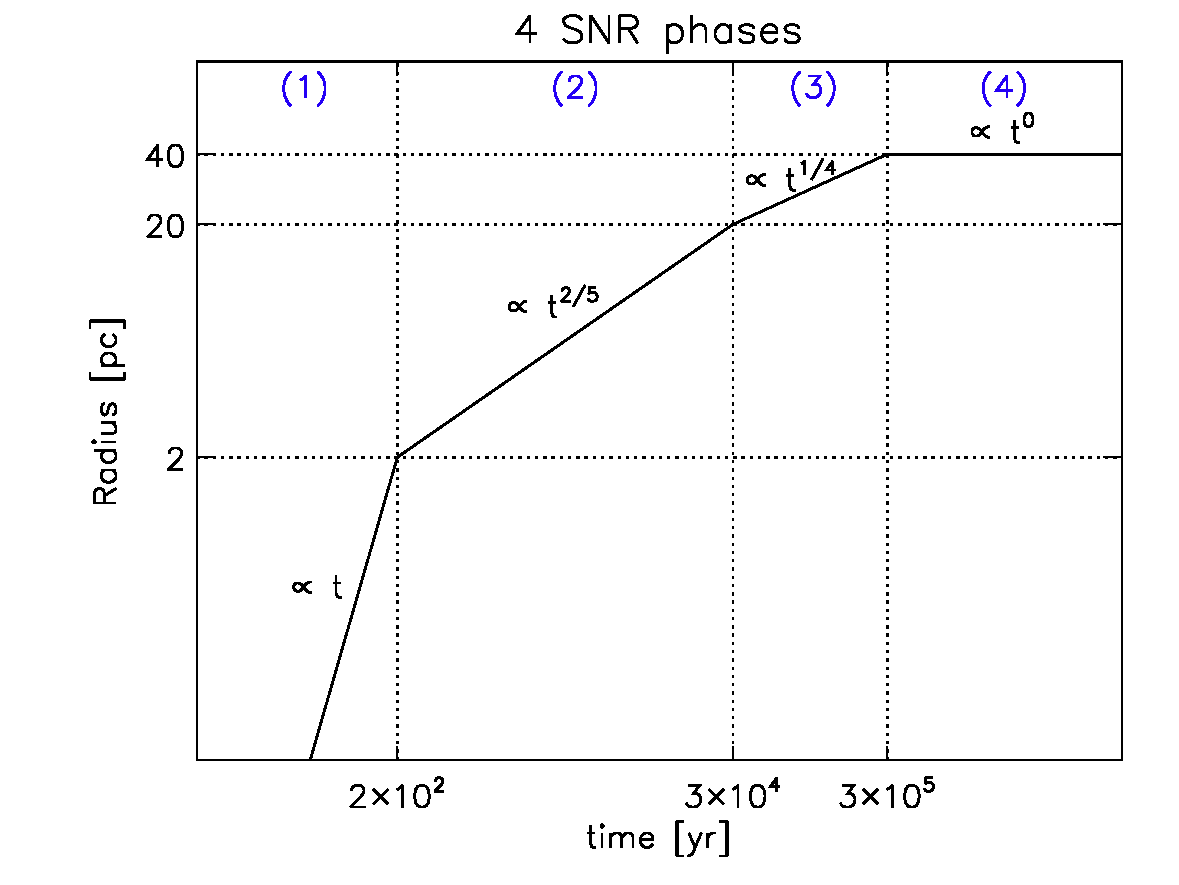
\includegraphics[width=0.7\textwidth]{HighEnergy/SNRphase}
    \caption{4 Supernova remnants phases: (1) free expansion (2) Sedov-Taylor expansion (3) Snowplow phase (4) relaxing phase.
            Note that x\&y axes are in logarithmic scale.}
    \label{fig:SNRphase}
\end{figure}

\noi (1) free expansion ($v=v_{\rm ej}=$constant)

The energy of supernova explosion is roughly:
\begin{equation}
    E_{\rm SN} \sim \frac{1}{2}\,M_{\rm ej}\,v_{\rm ej}^{2},
\end{equation}
where the ejected outflow velocity is,
\begin{equation}
    v_{\rm ej} \sim 10^{4}\, km/s \, \left( \frac{E_{\rm SN}}{10^{51}\,erg} \right)^{1/2} \left( \frac{M_{\rm ej}}{M_{\odot}} \right)^{-1/2}.
\end{equation}
The mass of swept-up gas becomes
\begin{equation}
    M_{\rm swept-up} \sim \frac{4\pi}{3}\,r^{3}\,\rho_{\rm ISM}.
\end{equation}
As a result, the bubble radius during this phase increases until $M_{\rm swept-up} \sim M_{\rm ej}$,
\begin{equation}
    r \sim 2\,pc\,\left( \frac{M_{\rm ej}}{M_{\odot}} \right)^{1/3} \left( \frac{\rho_{\rm ISM}}{10^{-24}\,g\,cm^{-3}} \right)^{-1/3},
\end{equation}
and the final time of this stage is
\begin{equation}
    t \sim \frac{r}{v_{\rm ej}} \sim 200\, yr\, \left( \frac{E_{\rm SN}}{10^{51}\,erg} \right)^{-1/2} \left( \frac{M_{\rm ej}}{M_{\odot}} \right)^{5/6}
                                 \left( \frac{\rho_{\rm ISM}}{10^{-24}\,g\,cm^{-3}} \right)^{-1/3}.
\end{equation}

\noi (2) Sedov-Taylor expansion ($E=E_{\rm SN}=$constant)

The energy is conserved in this stage: $E_{\rm SN} \propto M\,v^{2} \propto \rho_{\rm ISM}\,r^{3}\,\dot{r}^{2}$,
thereby
\begin{eqnarray}
    r^{3}\left( \frac{dr}{dt} \right)^{2} &\propto& \frac{E_{\rm SN}}{\rho_{\rm ISM}} \nonumnext
    r^{3/2}\,dr &\propto& \left( \frac{E_{\rm SN}}{\rho_{\rm ISM}} \right)^{1/2}\,dt \nonumnext
    \therefore r &\propto& \left( \frac{E_{\rm SN}}{\rho_{\rm ISM}} \right)^{1/5}\, t^{2/5} 
\end{eqnarray}

The typical outflow velocity is $\sim 200\, km/s$ and the temperature drops to $10^{6}\, K$, which emits
strong X-ray thermal bremsstrahlung.

\noi (3) Snowplow phase ($p$=constant)

The temperature drops below $10^{6}\, K$ so that radiative cooling becomes dominant by some recombination processes.
In this stage, the cold dense shell is driven by the hot interior. 
\begin{equation}
    \frac{d}{dt}(M\,v) = \frac{d}{dt}\left( \frac{4\pi}{3}\,\rho\,r^{3}\,\dot{r} \right) = 0.
\end{equation}
Assuming a thin shell forms at $t_{0}$ with the size of $r_{0}$ and the outflow velocity of $v_{0}$,
\begin{eqnarray}
    r^{3}\,\dot{r} &=& r_{0}^{3}\,v_{0} \nonumnext
    r &=& r_{0} \left[ 1 + \frac{4\,v_{0} (t-t_{0})}{r_{0}} \right]^{1/4}.
\end{eqnarray}

\noi (4) mixing phase with ISM ($r$=constant)

The typical temperature and outflow velocity are $10^{4}\, K$ and $10\, km/s$, respectively. 
The speed of ejecta becomes comparable to the sound speed of ISM.


\subsubsection{bubble with continuous energy injection:\\ (bubble at pulsars or microquasars)}

The solution for the expanding shock front supported by spin-down energy from central pulsar
wind must be a scale-free or self-similar solution, which can be expressed of the dimensionless
variable, $\eta$, where

\begin{equation}
   \eta \equiv r\,t^{l}\,\rho_{0}^{m}\,\dot{E_{0}}^{n},
\end{equation}

\noi the exponents $l$,$m$, and $n$ are determined by the requirement that $\eta$ is
dimensionless.  Since the $\dot{E_{0}}$ has the dimensionality $M\,L^{2}\,T^{-3}$, and the
$\rho_{0}$ has the dimensionality $M\,L^{-3}$, the dimensionality of $\eta$ should be
$L^{1-3m+2n}\,T^{l-3n}\,M^{m+n}$. Therefore, the exponents $l=-3/5, m=1/5,$ and $n=-1/5$,

\begin{equation}
   \eta = r \, \left( \frac{\rho_{0}}{\dot{E_{0}}t^{3}} \right)^{1/5},
\end{equation}

\noi or,

\begin{equation}\label{eq:Rs}
   R_{s}(t) = \eta \left( \frac{\dot{E_{0}}}{\rho_{0}} \right)^{1/5}\,t^{3/5}.
\end{equation}

In order to calculate the normalized factor, $\eta$, descriptions in \cite{Castor:75}
are adopted. In their notation, region b indicates a hot, almost isobaric region consisting 
of shocked stellar wind, and region c indicates a thin, dense, cold shell at radius,$R_{s}$
expending at velocity $\dot{R_{s}}$, and containing most of the swept-up ISM gas.

The dominant energy loss of region b is work against the dense shell, region c, so that the
total energy of region b should be

\begin{equation}\label{eq:Castor1}
   \dot{E_{b}} = \dot{E_{0}} - 4 \pi R_{s}^2 P_{b} \dot{R_{s}},
\end{equation}

\noi with

\begin{equation}\label{eq:Castor2}
   \frac{4}{3} \pi R_{s}^3 P_{b} = \frac{2}{3} E_{b}.
\end{equation}

In addition, the motion of the shell, region c, follows from 

\begin{equation}\label{eq:Castor3}
   \frac{d}{dt} \left[ M_{c}(t) \dot{R_{s}}(t) \right] = 4 \pi R_{s}^{2} P_{b},
\end{equation}

\noi where

\begin{equation}\label{eq:Castor4}
   M_{c}(t) = \frac{4}{3}\pi \rho_{0} R_{s}^3,
\end{equation}

\noi assuming that most of the swept-up interstellar mass remains in the shell. Combining eq. 
(\ref{eq:Castor1})-(\ref{eq:Castor4}) allows us to derive the radial evolution of the shell.
As we differentiate eq. (\ref{eq:Castor2}),

\begin{equation}
   \dot{E_{b}} = 6 \pi R_{s}^{2} \dot{R_{s}} P_{b} + 2 \pi R_{s}^3 \dot{P_{b}},
\end{equation}

\noi and combine it with eq. (\ref{eq:Castor1}),

\begin{equation}\label{eq:Castor1-1}
  \therefore \, 10 \pi R_{s}^{2} \dot{R_{s}} P_{b} + 2 \pi R_{s}^{3} \dot{P_{b}} = \dot{E_{0}}
\end{equation}

Meanwhile, eq. (\ref{eq:Castor3})\&(\ref{eq:Castor4}) can be further calculated as, 

\begin{eqnarray}\label{eq:Castor4-1}
   \frac{d}{dt} \left[ \frac{4}{3}\pi R_{s}^3 \rho_{0} \dot{R_{s}} \right] &=& 4 \pi R_{s}^2 P_{b} \nonumnext
   \rightarrow \, 3 \dot{R_{s}^2} + R_{s} \ddot{R_{s}} &=& 3 \frac{P_{b}}{\rho_{0}}.
\end{eqnarray}

For the purpose of simplification, we substitute $\eta \left( \frac{\dot{E_{0}}}{\rho_{0}}
\right)^{1/5} \equiv A$, where $A$ is constant, then we set eq. (\ref{eq:Rs}) to $R_{s}(t) =
A \, t^{3/5}$. Plugging it into eq. (\ref{eq:Castor4-1}) allows us to express $P_{b}$ as,

\begin{equation}\label{eq:Pb}
   P_{b} (t) = \frac{7}{25} A^{2} \, \rho_{0} \, t^{-4/5},
\end{equation}

Finally we plug eq. (\ref{eq:Pb}) into eq.(\ref{eq:Castor1-1}), we get

\begin{eqnarray}
   \frac{154}{125} \pi A^{5} \rho_{0} &=& \dot{E_{0}}  \nonumnext
   \therefore \, A &=& \left( \frac{\dot{E}}{\rho_{0}} \right)^{1/5} \left( \frac{125}{154 \pi} \right)^{1/5}
\end{eqnarray}

\noi or equivalently,

\begin{equation}\label{eq:eta}
   \eta = \left( \frac{125}{154 \pi} \right)^{1/5}.
\end{equation}

\bigskip
\subsection{Accretion Disk}
\subsubsection{overview}
In the 1960s, X-ray observations and radio imaging of cosmic sources led to the realization 
that compact objects are a) numerous and b) extremely bright and c) extremely luminous. Understanding
what powers these sources required the formulation of a theory of accretion.

Beyond  high energy astrophysics, accretion is important in many other scenarios, such as star formation
and growth of starcluster.

\begin{itemize}
\item Arguments for accretion onto compact objects:\\
Consider a cosmic X-ray source (either an X-ray binary or an AGN).

\subitem AGN: Observe $L_{bol}\approx 10^{45}-10^{46} ~\unitpower$ \\
     $~~~~~~~~~~~~~~~$Observe variability with $\Delta \tau \sim \rm\,hours - years$
\subitem XRB: Observe $L_{bol}\approx 10^{38} ~\unitpower$ \\
     $~~~~~~~~~~~~~~~$Observe variability with $\Delta \tau \sim 10^{-3} - 1 \rm\,sec$

\item Causality: For a stationary object emitting with considerable variability on timescale
$\Delta \tau$ (with $\ge$ 50 \% $\Delta L$), we infer a size unit of
\begin{equation}
   R_{obj} \le \Delta \tau \cdot c,
\end{equation}
from causality arguments (significant portion of the object must light up within $\Delta \tau$, and light
travel time across object must, therefore, be $\le \Delta \tau$)

$\Rightarrow \rm\,R_{AGN} \le$ AU to PC

$~~~~\rm\,R_{XRB} \le \, 100\,km\, to~ R_{\odot}$

\item Efficiency: Suppose the object is powered by consuming some fuel at some rate $\dot{M}$ and converting to radiation 
with some efficiency $\eta$:

\begin{equation}
   L = \eta \dot{M} c^{2},
\end{equation}
so,
\begin{eqnarray}
   \dot{M} = \frac{L}{\eta c^{2}} &=& 1.4\times10^{18}\,\unitmflux \left( \frac{L}{10^{38}\,\unitpower} \right) \left( \frac{10\%}{\eta} \right) \nonumnext
                                  &\cong& 2\times10^{-8} \,\unitmfluxsol \left( \frac{L}{10^{38}\, \unitpower} \right) \left( \frac{10\%}{\eta} \right)
\end{eqnarray}

\item Characteristic masses: Dynamical mass estimates are available for both AGN and XRBs

\[ \left. 
\begin{array}{rl}
M_{AGN} & \sim 10^{6} - 10^{10} \, M_{\odot}  \\ 
M_{XRB} & \sim 1 - 30 \, M_{\odot}  
\end{array}
\right\} ~ \textrm{\bf Compact Object !}  \]

\item Possible power sources:

\subitem a) Chemical: $\eta_{chem} \approx \rm eV/nucleon \approx 10^{-9}$
\subitem b) Nuclear: $\eta_{nuc} \approx \rm MeV/nucleon \approx 10^{-3}$
\subitem c) accretion:
\begin{eqnarray}
 R_{isco} &=& \frac{6GM}{c^{2}} \nonumnext
 \Delta{E_{isco}} &=& \frac{1}{2} \frac{GM m_{p}}{R_{isco}}=\frac{GM m_{p} c^{2}}{12 GM} = \frac{m_{p}c^{2}}{12} \nonumnext
 \rightarrow \eta_{acc} &\approx& \frac{1}{12} \approx 10\,\% \approx 100\times \eta_{nuc} \approx 10^{8} \eta_{chem} \nonumber
\end{eqnarray}
$~~~~~~~~$ accretion by far the most efficient power source.

\item Growth time: 
\begin{equation}
   T_{\dot{M}} = \frac{M}{\dot{M}} = 4 \times 10^{7}\, yrs \left(\frac{\eta}{10\%}\right) \left(\frac{M}{M_{\odot}}\right) \left(\frac{10^{38}\,erg\,s^{-1}}{L} \right)
\end{equation}

This immediately rules out chemical power and even a nuclear powered source with quickly run
out of fuel. We will formalize this argument further in the context of AGN.  

\end{itemize}

\subsubsection{How does accretion work?}

\textbf{Spherical/Bondi-Hoyle accretion}:  \\
Consider massive, gravitating compact object placed in a stationary, uniform medium 

$\Rightarrow$ no pressure gradients to support against gravity.

$\Rightarrow$ spherically symmetric infall (no preferred direction)

\begin{figure}[!htbp]
   \centering
   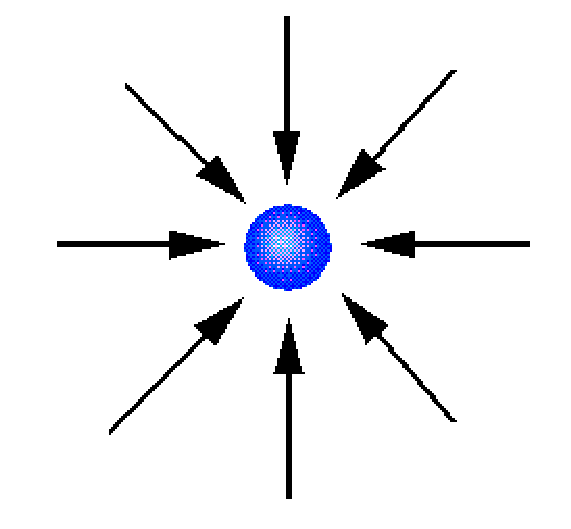
\includegraphics[width=0.25\textwidth]{HighEnergy/infall}
   \caption{sketch of spherical infall}
\label{fig:infall}
\end{figure}

Questions:

\begin{itemize}
   \item What is the structure of such a flow?
   \item How much gas is accreted at what rate?
   \item How much energy is released?
   \item what is the applicability of such a solution?
\end{itemize}

\textbf{ Order of magnitude estimates:}

The event horizon for a black hole is $2\frac{GM}{c^{2}} \equiv r_{s}$. Inside $r_{s}$, even
light, moving at c, is bound and must travel inward, the region inside is causally disconnected.
Regular matter is bound to black hole further out: For material with temperature T and sound
speed $c_{s} \approx \sqrt{kt/m_{p}}$, material is bound for

\begin{eqnarray}
   E_{thermal} &\le& E_{pot} \nonumnext
   \Leftrightarrow ~ kT = m_{p}c_{s}^{2} &\le& \frac{G M m_{p}}{r_{Bondi}}
\end{eqnarray}
\begin{equation}
   \therefore r_{Bondi} \sim \frac{GM}{c_{s}^2}
\end{equation}
,Bondi radius, is the capture radius of the black hole for gas at temperature T. Inside
$r_{Bondi}$, gas must be bound to the black hole.

Spherical accretion: no hydrostatic pressure support

$\Rightarrow ~~ v_{Bondi} \approx -c_{s}$

At $r_{Bondi}$, so for gas with density $\rho$, accretion rate is

\begin{eqnarray}
   \dot{M} &\approx& 4\pi R^{2}\rho v = 4\pi r_{Bondi}^2 \rho c_{s} \nonumnext
           &=& \frac{4\pi G^{2}M^{2}\rho}{c_{s}^3}
\end{eqnarray}
Note: $\dot{M} \propto M^{2}$ and $\dot{M} \propto c_{s}^{-3} \propto T^{-3/2}$.


\begin{enumerate}[a)]
   \item Stellar mass compact object: 

\begin{equation} 
   \dot{M}_{Bondi} \approx 5 \times 10^{11}\,g\,s^{-1} \left( \frac{M}{M_{\odot}} \right)^{2} \left( \frac{n_{ISM}}{1\,cm^{-3}} \right) \left( \frac{T}{10^{4}\,K} \right)^{-3/2}
\end{equation}
   For accretion at 10\% efficiency, luminosity is
\begin{equation}
   L_{Bondi} \approx 10^{31} \,\unitpower
\end{equation}

   \item Supermassive black holes:
\begin{eqnarray}
  \dot{M}_{Bondi} &\approx& 5\times10^{23} \unitmflux \left( \frac{M}{3 \times 10^{9}\,M_{\odot}} \right)^{2} 
                             \left( \frac{n}{10^{-2}\,cm^{-3}} \right) \left( \frac{c_{s}}{400\,\unitv} \right)^{-3} \nonumnext
                   &\approx& 2.5\times10^{-10} {\rm\,M_{\odot}\,s^{-1}} \approx 0.03\, \unitmfluxsol
\end{eqnarray}
   and again for 10\% efficiency:
\begin{equation}
   L_{Bondi} \approx 5\times10^{43} \unitpower \left( \frac{M}{M_{87}} \right)^{2}
                             \left( \frac{n}{10^{-2}\,cm^{-3}} \right) \left( \frac{c_{s}}{400\,\unitv} \right)^{-3}
\end{equation}

$\Rightarrow$ Bondi accretion might be sufficient for moderate AGN powers, it never works to
power XRBs. That's why we can't see isolated black holes of stellar mass inside our Galaxy, even if they exist.

$\therefore$ Need another source of matter for XRBs.

\textcolor{red}{Detailed solution of Bondi-Hoyle accretion }
\end{enumerate}

\textbf{Problems with spherical accretion:}
\begin{enumerate}[a)]
   \item Radiation pressure \\
         The radiative force on a particle is 
\begin{eqnarray}
    F_{rad} &=& \textrm{radiation momentum flux} \times \textrm{cross section} \nonumnext
                &=& \int d\nu \frac{F_{\nu}}{c} \sigma_{\nu}
\end{eqnarray}
For ionized gas, use $\sigma_{T}$ and $F = L/4\pi r^{2}$.

Radiation pressure becomes overwhelming when the radiative force exceeds the gravitational force:
\begin{equation}
   F_{rad} = \frac{L}{4\pi r^{2}} \frac{\sigma_{T}}{c} > \frac{GM}{r^{2}} m_{p}
\end{equation}
\begin{empheq}[innerbox=\fbox,
left=\Leftrightarrow]{align}
L>L_{\rm Edd} = \frac{GM m_{p} 4\pi c}{\sigma_{T}} = 1.3\times10^{38}\,\unitpower \left( \frac{M}{M_{\odot}} \right)
\end{empheq}
where $L_{Edd}$ is Eddington Luminosity. Note that $L_{Edd}$ is independent of $r$
and can be higher for non-ionized, heavy particles.

For an accretion efficiency of 10\%, $L_{Edd}$ corresponds to an accretion rate of 
\begin{eqnarray}
  \dot{M}_{Edd} &=& \frac{L_{Edd}}{0.1\,c^{2}} \nonumnext
                &=& 1.4\times10^{18}\,\unitmflux \,M/M_{\odot} = 2\times10^{-8} \,\unitmfluxsol\,M/\unitmsun
\end{eqnarray}

  \item Angular momentum
  
The assumption of spherical symmetry is almost always incorrect: any realistic gas reservoir will have net angular momentum
with respect to accreting object.

$\Rightarrow$ centrifugal barrier prevents radial infall

\begin{figure}[!htbp]
   \centering
   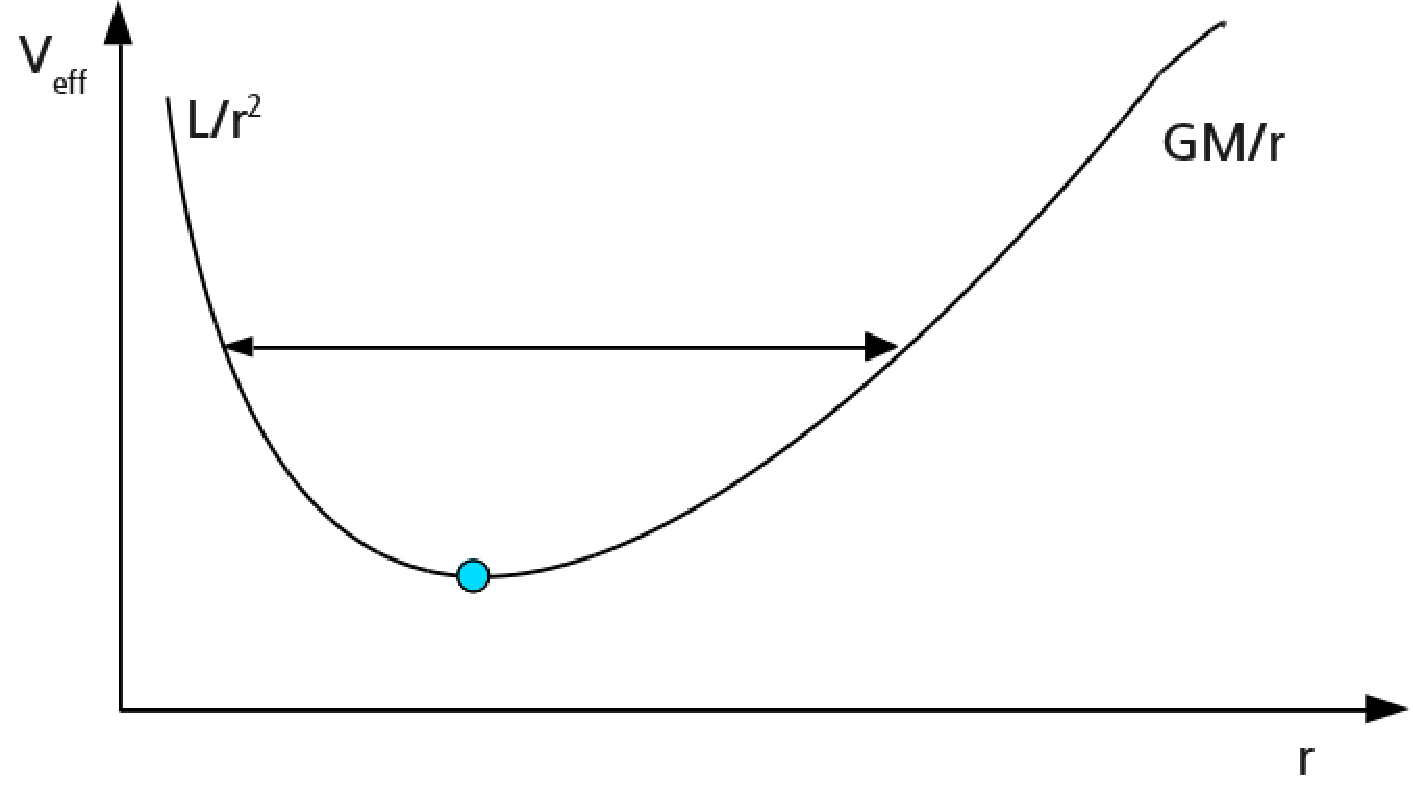
\includegraphics[width=0.7\textwidth]{HighEnergy/angplot}
   \caption{Effective energy with angular momentum, L. Circular orbit will be taken at minimum energy for given L.}
\label{fig:angplot}
\end{figure}

$\Rightarrow$ Crossing eccentric orbits dissipate and circularize.

No centrifugal barrier in vertical direction to counteract z-component of gravity: \textbf{disk formation}
\end{enumerate}

\begin{figure}[!htbp]
   \centering
   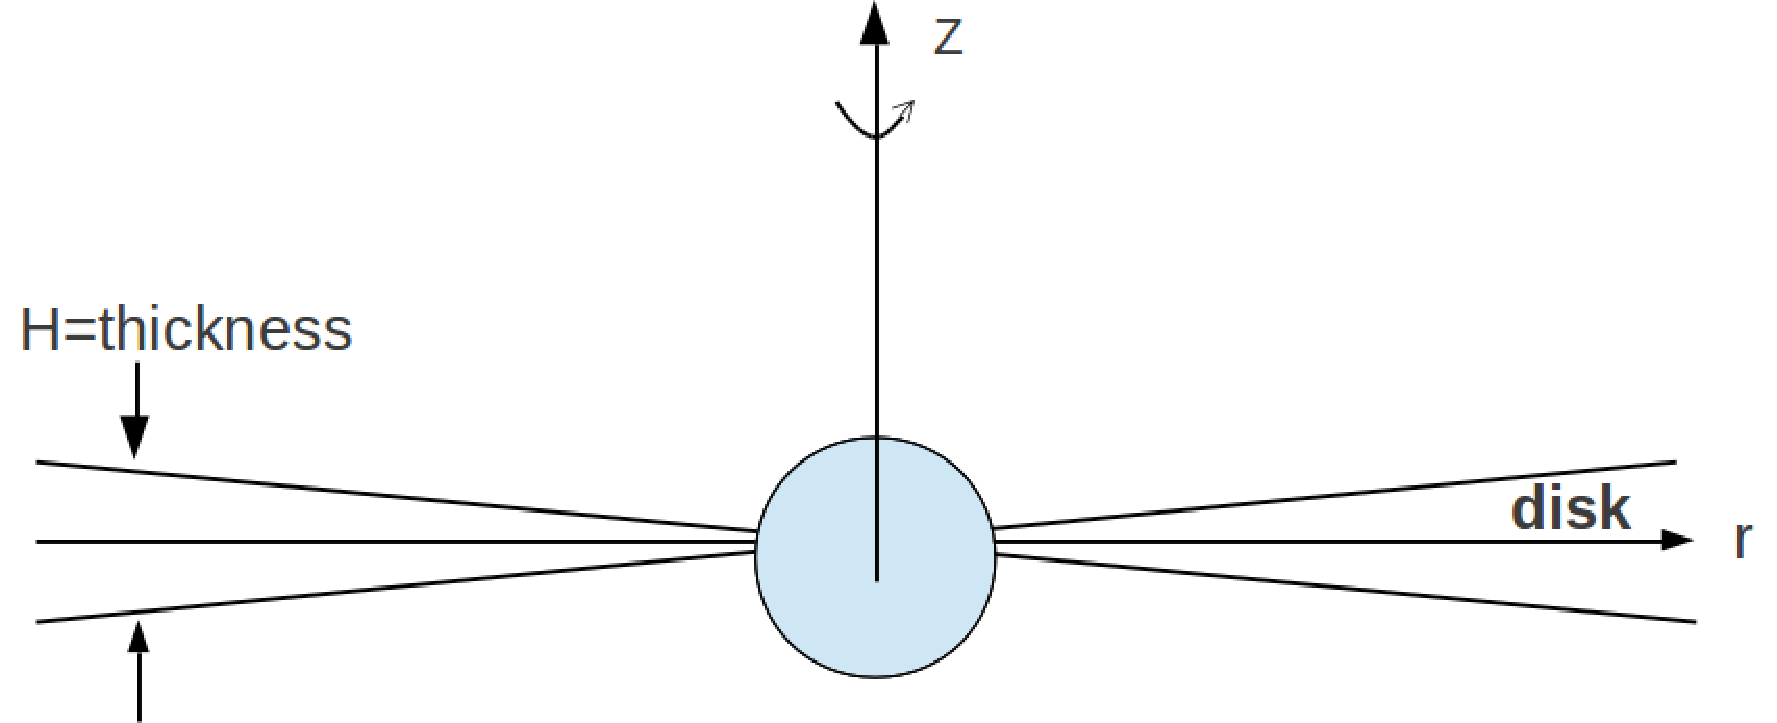
\includegraphics[width=0.7\textwidth]{HighEnergy/disk}
   \caption{Sketch of accretion disk. Centered object will be black hole or neutron star, \ldots. $F_{z}\cong \frac{GM}{r^{2}} \frac{z}{r}$}
\label{fig:disk}
\end{figure}

\textbf{Vertical hydrostatic balance:}

$\Rightarrow$ Only pressure gradient balances vertical gravity.

\begin{figure}[!htbp]
   \centering
   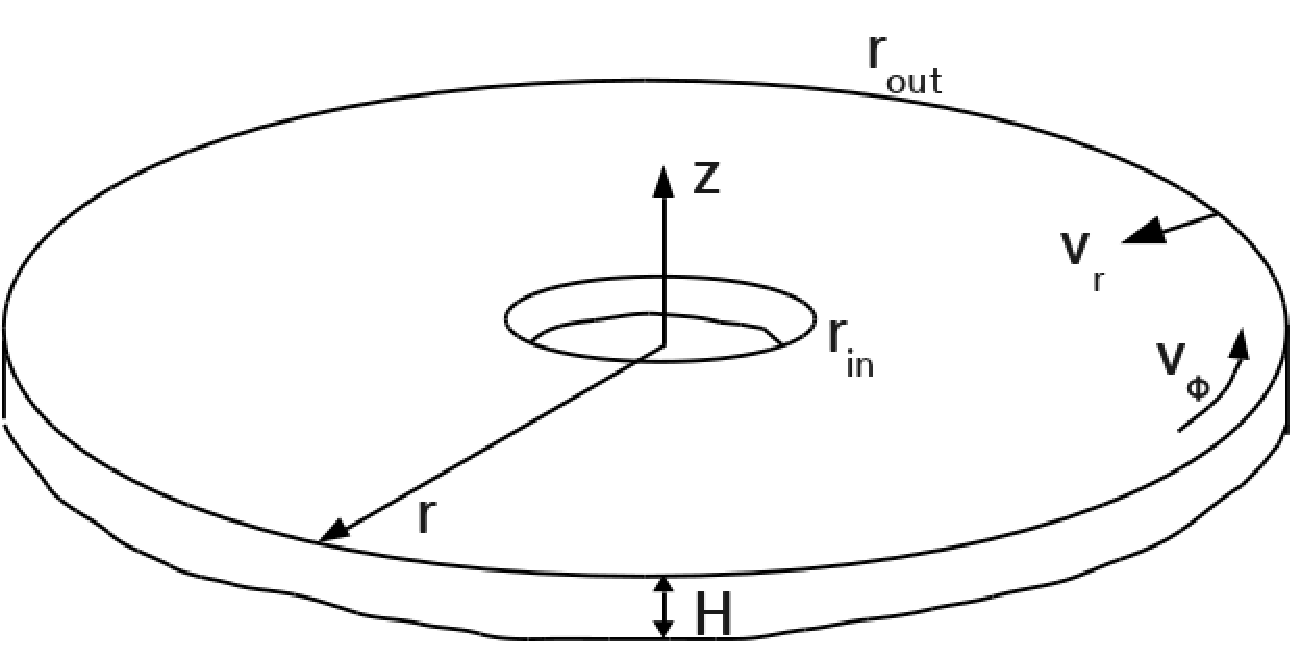
\includegraphics[width=0.7\textwidth]{HighEnergy/accretion}
   \caption{Hydrostatic balance in accretion disk.}
\label{fig:accretion}
\end{figure}

\begin{eqnarray}
   r \Omega &=& v_{\phi} \\
   r \Omega^{2} &=& \frac{GM}{r^{2}}
\end{eqnarray}

\textcolor{red}{
\begin{equation}
   (\text{cf. }L=r^{2}\Omega = r^{2} \sqrt{\frac{GM}{r^{3}}} \propto r^{1/2} ~~\text{for keplerian disk})
\end{equation}
}

The pressure gradient in vertical direction will be balanced by the gravity via
\begin{equation}
   \nabla_{z}P = \frac{\partial}{\partial z}P = \rho g_{z} = -\frac{GM\rho}{r^{2}} \frac{z}{r} = -\rho \Omega^{2}z
\end{equation}

Ansatz: $H \ll r$ and $v_{r} \ll v_{\phi}$.

\begin{equation}
   \Rightarrow ~ \frac{\partial P}{\partial z} \approx -\frac{P}{H} = - \rho \Omega^{2} z \approx -\rho \Omega^{2} H
\end{equation}

\begin{equation}\label{eq:vhse}
   \Leftrightarrow ~ \frac{P}{\rho} \approx \Omega^{2} H^{2} = R^{2} \Omega^{2} \left( \frac{H^{2}}{R^{2}} \right)
   = v_{\phi}^2 \left( \frac{H}{R} \right)^2
\end{equation}
\begin{empheq}[innerbox=\fbox,
left=\Leftrightarrow]{align}
\left( \frac{c_{s}^2}{v_{\phi}^2} \right) \approx \left( \frac{H}{R} \right)^2
\end{empheq}
\begin{equation}
  \Rightarrow ~   v_{\phi} \gg c_{s}  ~\Leftrightarrow~ r \gg H
\end{equation}

Note that assumption of this model is 1) steady state ($\partial / \partial t = 0$), 2) $r \gg H$,and 3) $v_{\phi} \gg v_{r}$.

$\therefore$ Thin accretion disks ($H \ll r$) must be cold ($c_{s} \ll v_{\phi}$).

Also note that a virialized flow would have $c_{s} \approx v_{\phi}$.

\textbf{Order of Magnitude Scaling:}

\begin{enumerate}[a)]
   \item Mass conservation:

   From continuity equation (eq.(\ref{eq:continuity1})), mass transfer rate can be roughly estimated as

\begin{equation}
   \dot{M} = -2\pi R\,H \rho\,v_{R} \equiv -2 \pi R\, \Sigma\, v_{R},
\end{equation}
where $\Sigma$ is surface density. The factor 2 in the equation can be derived by second term in eq.(\ref{eq:continuity1}).
\begin{empheq}[innerbox=\fbox,
left=\Rightarrow]{align}
 \dot{M} \propto R\,\Sigma\,v_{R}
\end{empheq}

   \item Vertical hydrostatic balance:

From the relation ship in eq.(\ref{eq:vhse}),

\begin{equation}
 \Rightarrow ~ \frac{P}{\rho} \sim c_{s}^{2} \propto \Omega^{2} H^{2} \propto v_{\phi}^{2} \left( \frac{H}{R} \right)^2
\end{equation}
\begin{empheq}[innerbox=\fbox,
left=\Rightarrow]{align}
 T \propto \Omega^{2} H^{2}
\end{empheq}
where T is gas pressure dominated temperature in the accretion disk.

   \item Angular momentum conservation:

Advection will be produced by torque
\begin{equation}
  \dot{M} R^{2} \Omega \approx \underbrace{2\pi R\,H}\cdot\underbrace{R}\cdot\underbrace{\rho \nu \frac{\partial \Omega}{\partial R}\,R}
\end{equation}
where LHS is given by derivation of angular momentum, $\partial L / \partial t =\partial
(M\,R^{2}\Omega )/ \partial t$, and in RHS, first term is surface area and second term is lever arm and 
third term is viscous stress. The angular momentum will be transported to outward by viscosity.
\begin{empheq}[innerbox=\fbox,
left=\therefore ~]{align}
 \dot{M} \propto \Sigma\,\nu
\end{empheq}

\item Energy conservation:

Sources = Sinks  ~  ($Q^{+} = Q^{-}$)

Here sources can be gravity and the sinks can be radiation, advection(neglect for now).
\begin{eqnarray}
  Q^{+} &\sim& \frac{d\,E_{pot}}{dt\,dR}dR ~\sim \frac{GM\dot{M}}{R^{2}}dR \\
  Q^{-} &\sim& 2\pi R\,dR \cdot F \sim 2\pi R\,dR \cdot \sigma T_{eff}^{4}
\end{eqnarray}
Under the cool disk assumption, the flux will be dominant for blackbody radiation due to high opacity.
\begin{equation}
   \Rightarrow  ~ T_{eff}^{4} \propto \frac{GM\dot{M}}{R^{3}} \propto \Omega^{2}\dot{M} \propto M\dot{M}R^{-3}
\end{equation}
Interested in $T_{\rm central}$: Optically thick radiation
\begin{figure}[!htbp]
   \centering
   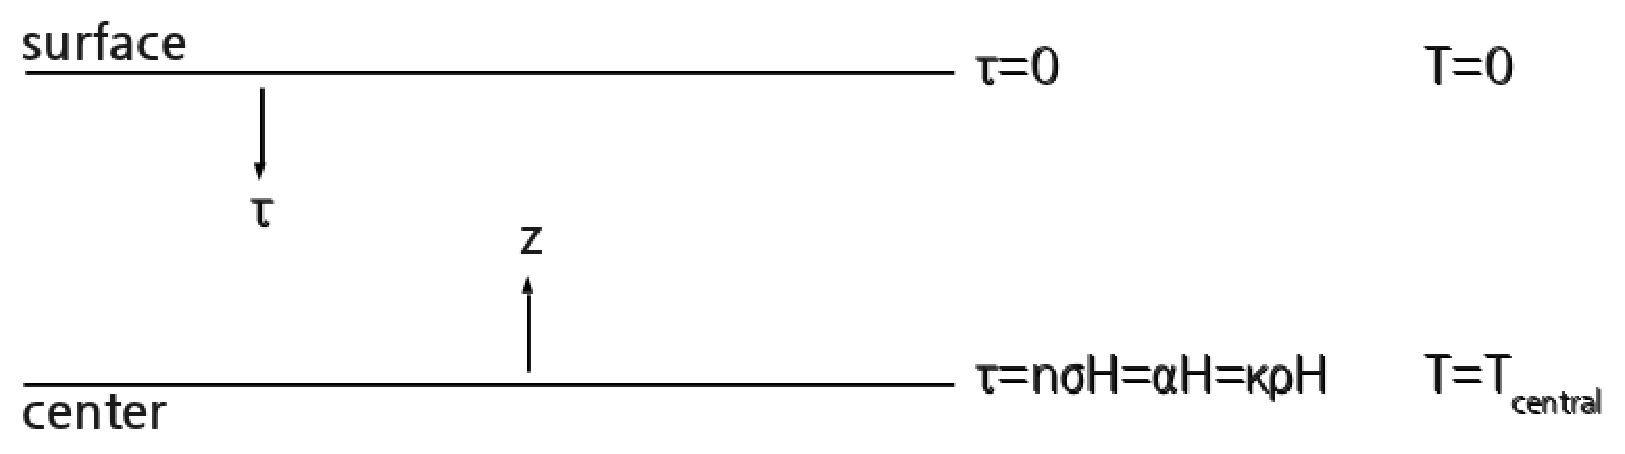
\includegraphics[width=0.7\textwidth]{HighEnergy/thickrad}
   \caption{Sketch of optical depth through disk}
\end{figure}
Radiation escapes from $\tau \le 1$
\begin{equation}
\Rightarrow ~ T_{\rm eff}^{4} \approx T_{\tau=1}^{4} \approx \frac{dT^{4}}{d\tau}\tau_{=1}
\approx \frac{4 T_{central}^4}{\tau_{central}} \approx \frac{4 T_{c}^4}{\kappa \rho H}
\end{equation}
\begin{empheq}[innerbox=\fbox,
left=\therefore ~]{align}
 \frac{T_{c}^4}{\kappa \rho H} \propto \Omega^{2} \dot{M}
\end{empheq}
Note that $\rho H = \Sigma$, so $T_{c}^{4} \propto \kappa \Sigma \Omega^{2} \dot{M}$.

And we will use Kramer's opacity, which is blackbody-weighted absorption.
\begin{empheq}[innerbox=\fbox]{align}
 \kappa_{kr} \propto \rho T^{-7/2} \propto \frac{\Sigma}{H}T^{-7/2}
\end{empheq}

   \item Viscosity: $\nu$ 
\begin{itemize}
   \item Describe microscopic transport of momentum
   \item Characterized by typical transport velocity $\tilde{v}$ and typical random step size $\lambda$:
\begin{equation}
   \nu \approx \lambda \tilde{v}
\end{equation}
   \item Molecular viscosity (kinetic theory):
\begin{equation}
   \nu \approx \lambda_{mfp} c_{s}
\end{equation}
where $\lambda_{mfp}$ is characteristic length of mean free path.

For astrophysical systems of size $l$, often $\lambda_{mfp} \ll l$
\begin{equation}
  \Rightarrow \textrm{Re} \equiv \frac{\textrm{inertial~transport}}{\textrm{viscous~transport}} = \frac{l\,v}{\lambda_{mfp} \cs} \gg 1
\end{equation}
where Re is the Reynolds number.

$\Rightarrow$~~ \textbf{Turbulence !!!!!}

\begin{figure}[!htbp]
   \centering
   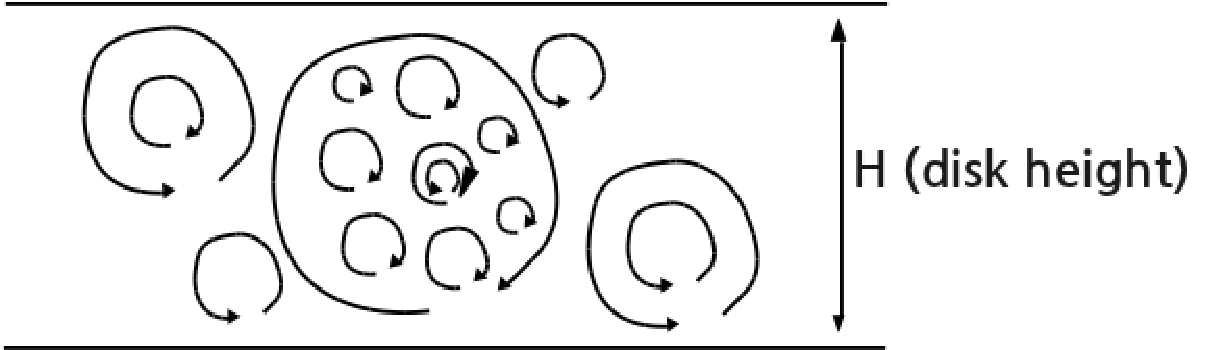
\includegraphics[width=0.7\textwidth]{HighEnergy/eddie}
   \caption{Eddies in the accretion disk. Characteristic length scale is maximum eddie size ($l \approx \rm H$).}
\end{figure}

  \item Characteristic speed: sound speed, $\tilde{v} \approx c_{s}$.
\begin{empheq}[innerbox=\fbox,
left=\therefore ~]{align}
    \nu \equiv \alpha c_{s} {\rm H}, ~~~~ \alpha \le 1
\end{empheq}
Which is \textbf{$\alpha$-disk model}.

   \item viscosity continued: \\
         $\alpha$ contains all uncertainties about $\nu$ very likely smaller than unity ($\alpha \le 1$).
         Very convenient, but \ldots
\end{itemize}
\end{enumerate}

\textbf{Putting it all together:}
\[ \left. 
\begin{array}{ll}
  (1)~~ \dot{M} \sim R \Sigma v_{R} & \rm (mass~ conservation) \\
  (2)~~ H \sim T^{1/2}\Omega^{-1} & \rm (vertical~ structure) \\
  (3)~~ \nu \sim \alpha T^{1/2} H & \rm (\alpha-viscosity) \\
  (4)~~ \dot{M} \sim \Sigma \nu \sim \Sigma \alpha T^{1/2} H & \rm (angular~ momentum) \\
  (5)~~ \frac{T^{4}}{\kappa \Sigma} \sim \dot{M} \Omega^{2} & \rm (energy~ equation) \\
  (6)~~ \kappa \sim \Sigma\,T^{-7/2}H^{-1} & \rm (Kramer's~ opacity)
\end{array} \right. \]

\textbf{Solutions:}

\begin{empheq}[innerbox=\fbox]{align}
 \boldsymbol  T \sim \dot{M}^{3/10} \alpha^{-1/5} M^{1/4} R^{-3/4} \\
 \boldsymbol \Sigma \sim \dot{M}^{7/10} \alpha^{-4/5} M^{1/4} R^{-3/4} \\
 \boldsymbol v_{R} \sim \dot{M}^{3/10} \alpha^{4/5} M^{-1/4} R^{-1/4} 
\end{empheq}
where in the steps, we have used $\Omega \sim  M^{1/2} R^{-3/2}$.

\textbf{Conclusions:}

\begin{enumerate}[1)]
   \item $\alpha$ enters T only marginally.
   \item $v_{R} \sim R^{-1/4}$ but $c_{s} \sim R^{-3/8}$ \\
         $\Rightarrow ~~ \frac{v_{R}}{c_{s}} \equiv M \sim R^{1/8}$ \\
         $\Rightarrow ~~$ less and less supersonic at smaller radius
   \item $v_{R} \sim \alpha^{4/5}$ \\
         $\Rightarrow ~~$ advection becomes more important for large $\alpha$.
\end{enumerate}

\textbf{A complete algebraic solution gives:}

\begin{empheq}[innerbox=\fbox]{align}
  T_{c} &= 1.4\times 10^{4}\,K ~ \alpha^{-1/5} \dot{M}_{16}^{3/10} M^{1/4} R_{10}^{-3/4} f^{6/5}  \\
  v_{R} &= 2.7\times 10^{4}\,cm\,s^{-1} ~ \alpha^{4/5} \dot{M}_{16}^{3/10} M^{-1/4} R_{10}^{-1/4} f^{-14/5} \\
  \tau  &= 33 ~ \alpha^{-4/5} \dot{M}_{16}^{1/5} f^{4/5} \\
  H     &= 1.7\times 10^{8}\,cm ~ \alpha^{-1/10} \dot{M}_{16}^{3/20} M^{-3/8} R_{10}^{9/8} f^{3/5} \\
 \Sigma &=5.2\,g\,cm^{-2} ~ \alpha^{-4/5} \dot{M}_{16}^{7/10} M^{1/4} R_{10}^{-3/4} f^{14/5} 
\end{empheq}
with $\dot{M}_{16} = \dot{M} / 10^{16} \,g\,s^{-1},~M=M_{BH}/M_{\odot},~R_{10}=R/10^{10}\,cm$, \\
and $f=\left[ 1 - \beta \left( R_{i}/R \right)^{1/2} \right]^{1/4}$ where $\beta$ is a viscous coupling constant.\\
Note that $T_{\rm eff}^{4} \sim \Omega^{2} \dot{M} \sim M\dot{M}R^{-3}$, that is independent of $\alpha$!!

\textbf{Spectrum:}
\begin{figure}[!htbp]
   \centering
   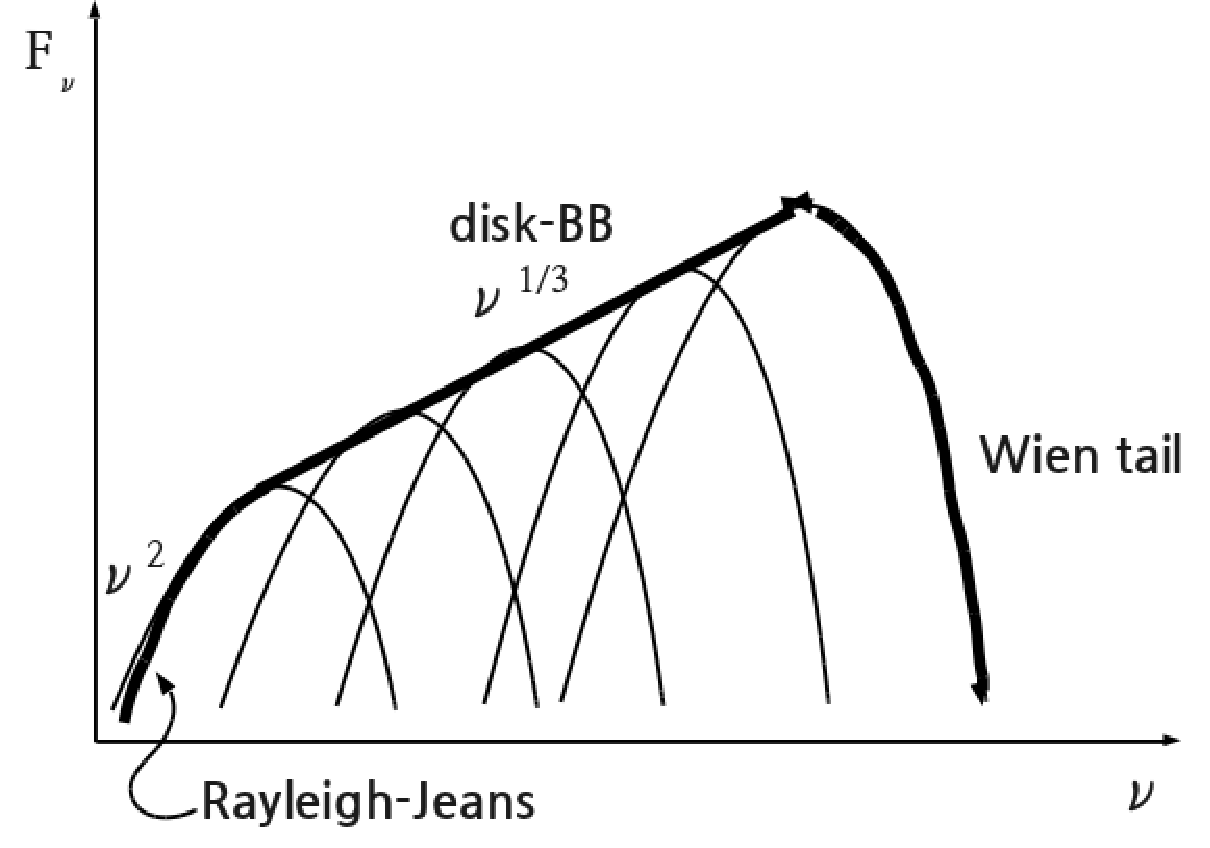
\includegraphics[width=0.65\textwidth]{HighEnergy/bhSpectrum}
   \caption{spectrum from accretion disk}
\end{figure}

The black body spectra from each part of accretion disk are superposed to produce characteristic spectrum.
The higher peak frequency of overlaid spectrum comes from inner disk. 
\[ \left. \begin{array}{ll}
  T_{\rm eff} = 1.3\times 10^{7} \,K ~ \dot{M}_{17}^{1/4} M^{1/4} R_{6}^{-3/4} & \textrm{(neutron star)} \\
  T_{\rm eff} = 1.3\times 10^{5} \,K ~ \dot{M}_{25}^{1/4} M_{8}^{1/4} R_{14}^{-3/4} & (10^{8}\,\unitmsun\,\textrm{black hole)} 
\end{array} \right. \]

\subsubsection{The role of magnetic fields: The magneto-rotational instability}

\begin{enumerate}[a)]
   \item The exact nature of the agent of angular momentum transport was unspecified (hidden in the $\alpha$-parameter)

   $\Rightarrow$~ Magnetic stresses could be responsible:

   A field line anchored into a ring at radius $r$ will co-rotate with this ring. It will try to speed up ring $r_{+}$(outer ring)
   and slow down ring $r_{-}$(inner ring).

   $\Rightarrow$~ angular momentum transport

   From MHD: magnitude of magnetic stress is $\frac{(\vec{B}\cdot\nabla)\vec{B}}{4\pi}$.

   Question: is $\frac{(\vec{B}\cdot\nabla)\vec{B}}{4\pi}$ sufficient, \ie, is B-field large enough?

   Answer: It will be, after a few Keplerian orbits.

   \item \textbf{Magneto-rotational instability (MRI):}

   Consider a vertical field line with a radial perturbation (fig.(\ref{fig:mrivt})).

\begin{figure}[!htbp]
   \centering
   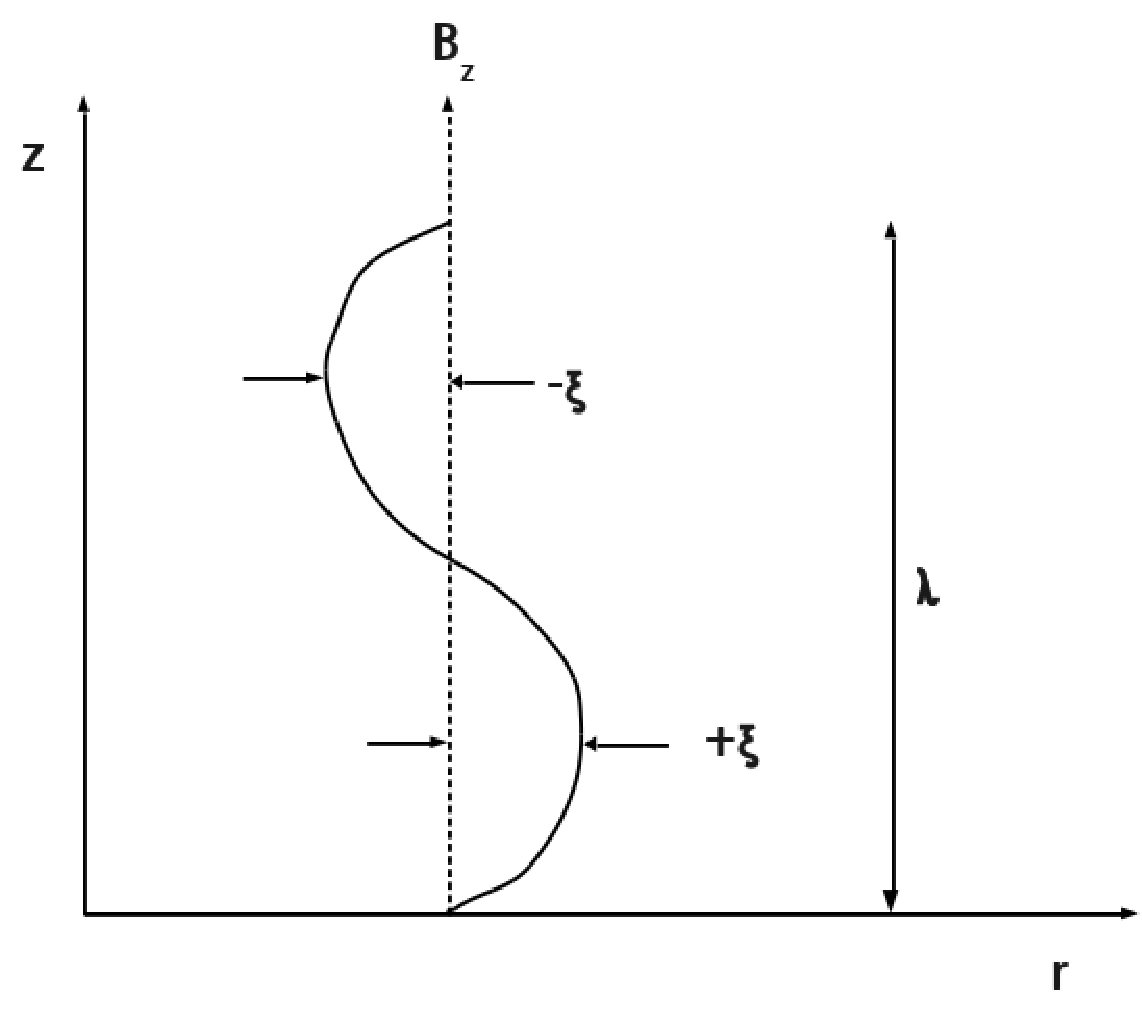
\includegraphics[width=0.7\textwidth]{HighEnergy/mrivt}
   \caption{Vertical magnetic field line}
   \label{fig:mrivt}
\end{figure}

   Here, wavelength $\lambda \le \rm H$ and amplitude(linear regime) $\xi \ll \lambda$.

   Magnetic force density in radial direction is (comment: $B_{r} \sim B_{z} \cdot \frac{\xi}{\lambda}$

\begin{equation}
   f_{B} = \frac{B_{z}}{4\pi}\frac{\partial}{\partial z}B_{r} \sim \frac{B_{z}}{4\pi}\left( - \frac{B_{r}}{\lambda} \right)
        \sim \frac{B_{z}^2}{4\pi}\left( - \frac{\xi}{\lambda^2} \right) \propto - \left( \vec{k}\cdot\vec{v}_{A} \right)^2 \rho\,\xi
\end{equation}
where $v_{A}$ is the \alfven speed, $v_{A}^2 = \frac{B_{z}^2}{4\pi\rho}$.
 
The net centrifugal force resulting from the perturbation is
\begin{equation}
   f_{c} = -\rho R \frac{\partial}{\partial R}(\Omega^{2})\xi = -\rho \frac{d\Omega^{2}}{d\,lnR}\xi
\end{equation}
The centrifugal force excess wins if
\begin{equation}
   f_{c}+f_{B} = -\rho \left( \frac{d \Omega^{2}}{d\,lnR} + \left( \vec{k}\cdot\vec{v}_{A}\right)^2 \right)\xi ~~ (>0\textrm{~for instability})
\end{equation}
which is positive for
\begin{equation}
    \frac{d \Omega^{2}}{d\,lnR} < - \left( \vec{k}\cdot\vec{v}_{A}\right)^2  ~~~ \Rightarrow ~ \textrm{instability}
\end{equation}
So there is a minimum wavelength (maximum $k$) for which the instability grows and we need
\begin{equation}
   \frac{d\Omega^{2}}{dR} < 0 
\end{equation}
with $\frac{B_{z}^{2}}{\lambda_{z}^{2}\rho} \le \Omega^{2}$ or $\lambda_{z}^2 \ge \frac{B_{z}^{2}}{\Omega^{2}\rho}$.
So unstable as long as ${\rm H} \ge \lambda_{\rm min}$ or ${\rm B} \le \textrm{equipartition}$.
(because $B^{2} \le {\rm H}^{2} \Omega^{2}\rho \le P$, where ${\rm H}^{2}\Omega^{2}=c_{s}^2$ in equipartition).

\end{enumerate}

\subsubsection{Other accretion regimes}

\noi We have neglected (among other things):

\begin{itemize}
   \item the inner boundary
   \item radiation pressure
   \item advection of energy
   \item time dependence
   \item non-local dissipation (B-fields), \ie, magnetic reconnection
\end{itemize}

\begin{enumerate}[a)]
   \item Radiation pressure:
   
\begin{equation}
   P_{\rm thermal} \propto T ~~~ vs. ~~~ P_{rad} \propto T^{4}
\end{equation}
   
Since, for the standard thin disk $T \sim \dot{M}^{3/10} \alpha^{-1/5} M^{1/4} R^{-3/4}$, the radiation 
pressure must dominate at large $\dot{M}$, small R.

It is straight forward to re-do the analysis by replacing the pressure term $\frac{a T^{4}}{3}$, but 
hardly worth is:

\textit{Radiation pressure supported disks are thermally and viscously unstable.}

$\Rightarrow$ equilibrium solution is never established.

Note: an accretion disk is anisotropic, so in principle, it can exceed the Eddington limit by a factor of a few.

   \item \textbf{Advection Dominated Accretion Flows (ADAFs)}

We have neglected energy advection $Q_{Adv}^{-}$ in the energy balance. The advective term becomes important
in (a) high $\dot{M}$ cases, where it can alleviate the Eddington limit and (b) low $\dot{M}$, high $\alpha$ cases.

Advection always decreases the radiative efficiency of the flow.

Advection dominated solution:
\begin{eqnarray}
   Q_{Adv}^{-} &\sim& \Sigma\,T\, 2\pi R v_{R} \sim T \dot{M} \\
   Q_{Adv}^{+} &\sim& \frac{G M \dot{M}}{R}
\end{eqnarray}

Balance:
\begin{equation}
  T \sim \frac{GM}{R}\sim \Omega^2 R^2 \sim T_{virial} ~~~\textrm{(hot)}
\end{equation}
and with vertical hydrostatic balance: $T\sim\Omega^2 H^2$
\begin{equation}
  H \sim T^{1/2} \Omega^{-1} \sim R ~~~ \rm (thick~disk~~ (cf.~ thin~ \leftarrow~ radiative~ dominate))
\end{equation}
so 
\begin{equation}
   v_{R} \sim \frac{\dot{M}}{\Sigma\,R}
\end{equation}
and
\begin{equation}
  \dot{M} \sim \Sigma \nu \sim \Sigma \alpha T^{1/2} H
\end{equation}
\begin{eqnarray}
   \Rightarrow ~~ v_{R} &\sim& \frac{\dot{M}}{\Sigma R} \sim \frac{\Sigma \alpha T^{1/2} H}{\Sigma R} 
                            \sim \alpha T^{1/2}H/R \nonumnext
                        &\sim& \alpha\Omega R \sim \alpha v_{\phi} ~~~~~~~~~~~~~(\textrm{rapid inflow})
\end{eqnarray}
Thus: Advection Dominated Accretion Flows are
\begin{itemize}
   \item hot (roughly at Virial temperature), $T \sim T_{\rm vir}$
   \item thick (not so much disk-like, more spherical), H$\,\sim\,$R
   \item non-Keplerian  (radial velocity comparable to $v_{\phi}$)
   \item require large $\alpha$
\end{itemize}
Note: ADAFs require radiative losses to be inefficient.

In a hot flow, it is possible that ions and electrons are thermally decoupled. If the ions get heated,
they might not transfer their energy to the electrons, who do all the radiating

$\Rightarrow$ ~~ Very hot flow implies strong Compton emission

$\Rightarrow$ ~~ Power-law emission (low-hard state ?)

As of today, it is not clear whether electrons and ions are really that strongly decoupled.

   \item The inner boundary: \\
We have neglected entirely what happens at the inner boundary. Introduces correction
\textcolor{red}{$\vartheta(r_{i}/r)$}\ldots

\begin{enumerate}[i)]
\item Neutron stars; WDs:

   Boundary layer must spin incoming material up or down to co-rotate with NS $\Rightarrow$ dissipation.

   Residual kinetic and thermal energy must be dissipated and radiated (\ie, no true advection).

\item Black holes:

   Usual assumption: zero-torque at marginally stable circular orbit (still introduces correction of order
   $r_{i}/r$ to solution)

   Energy can be advected across horizon.

   $\Rightarrow$ are low luminosity sources advection dominant?

   $\Rightarrow$ are black holes in quiescence dimmer than NS in quiescence because they have an event horizon? 

But note: \textbf{``The absence of evidence is not the evidence of absence.}

In other words, black holes could be dim for other reasons, their dimness is no proof for the
existence of event horizons (sadly, some might say) \end{enumerate}


\begin{figure}[!htbp]
   \centering
   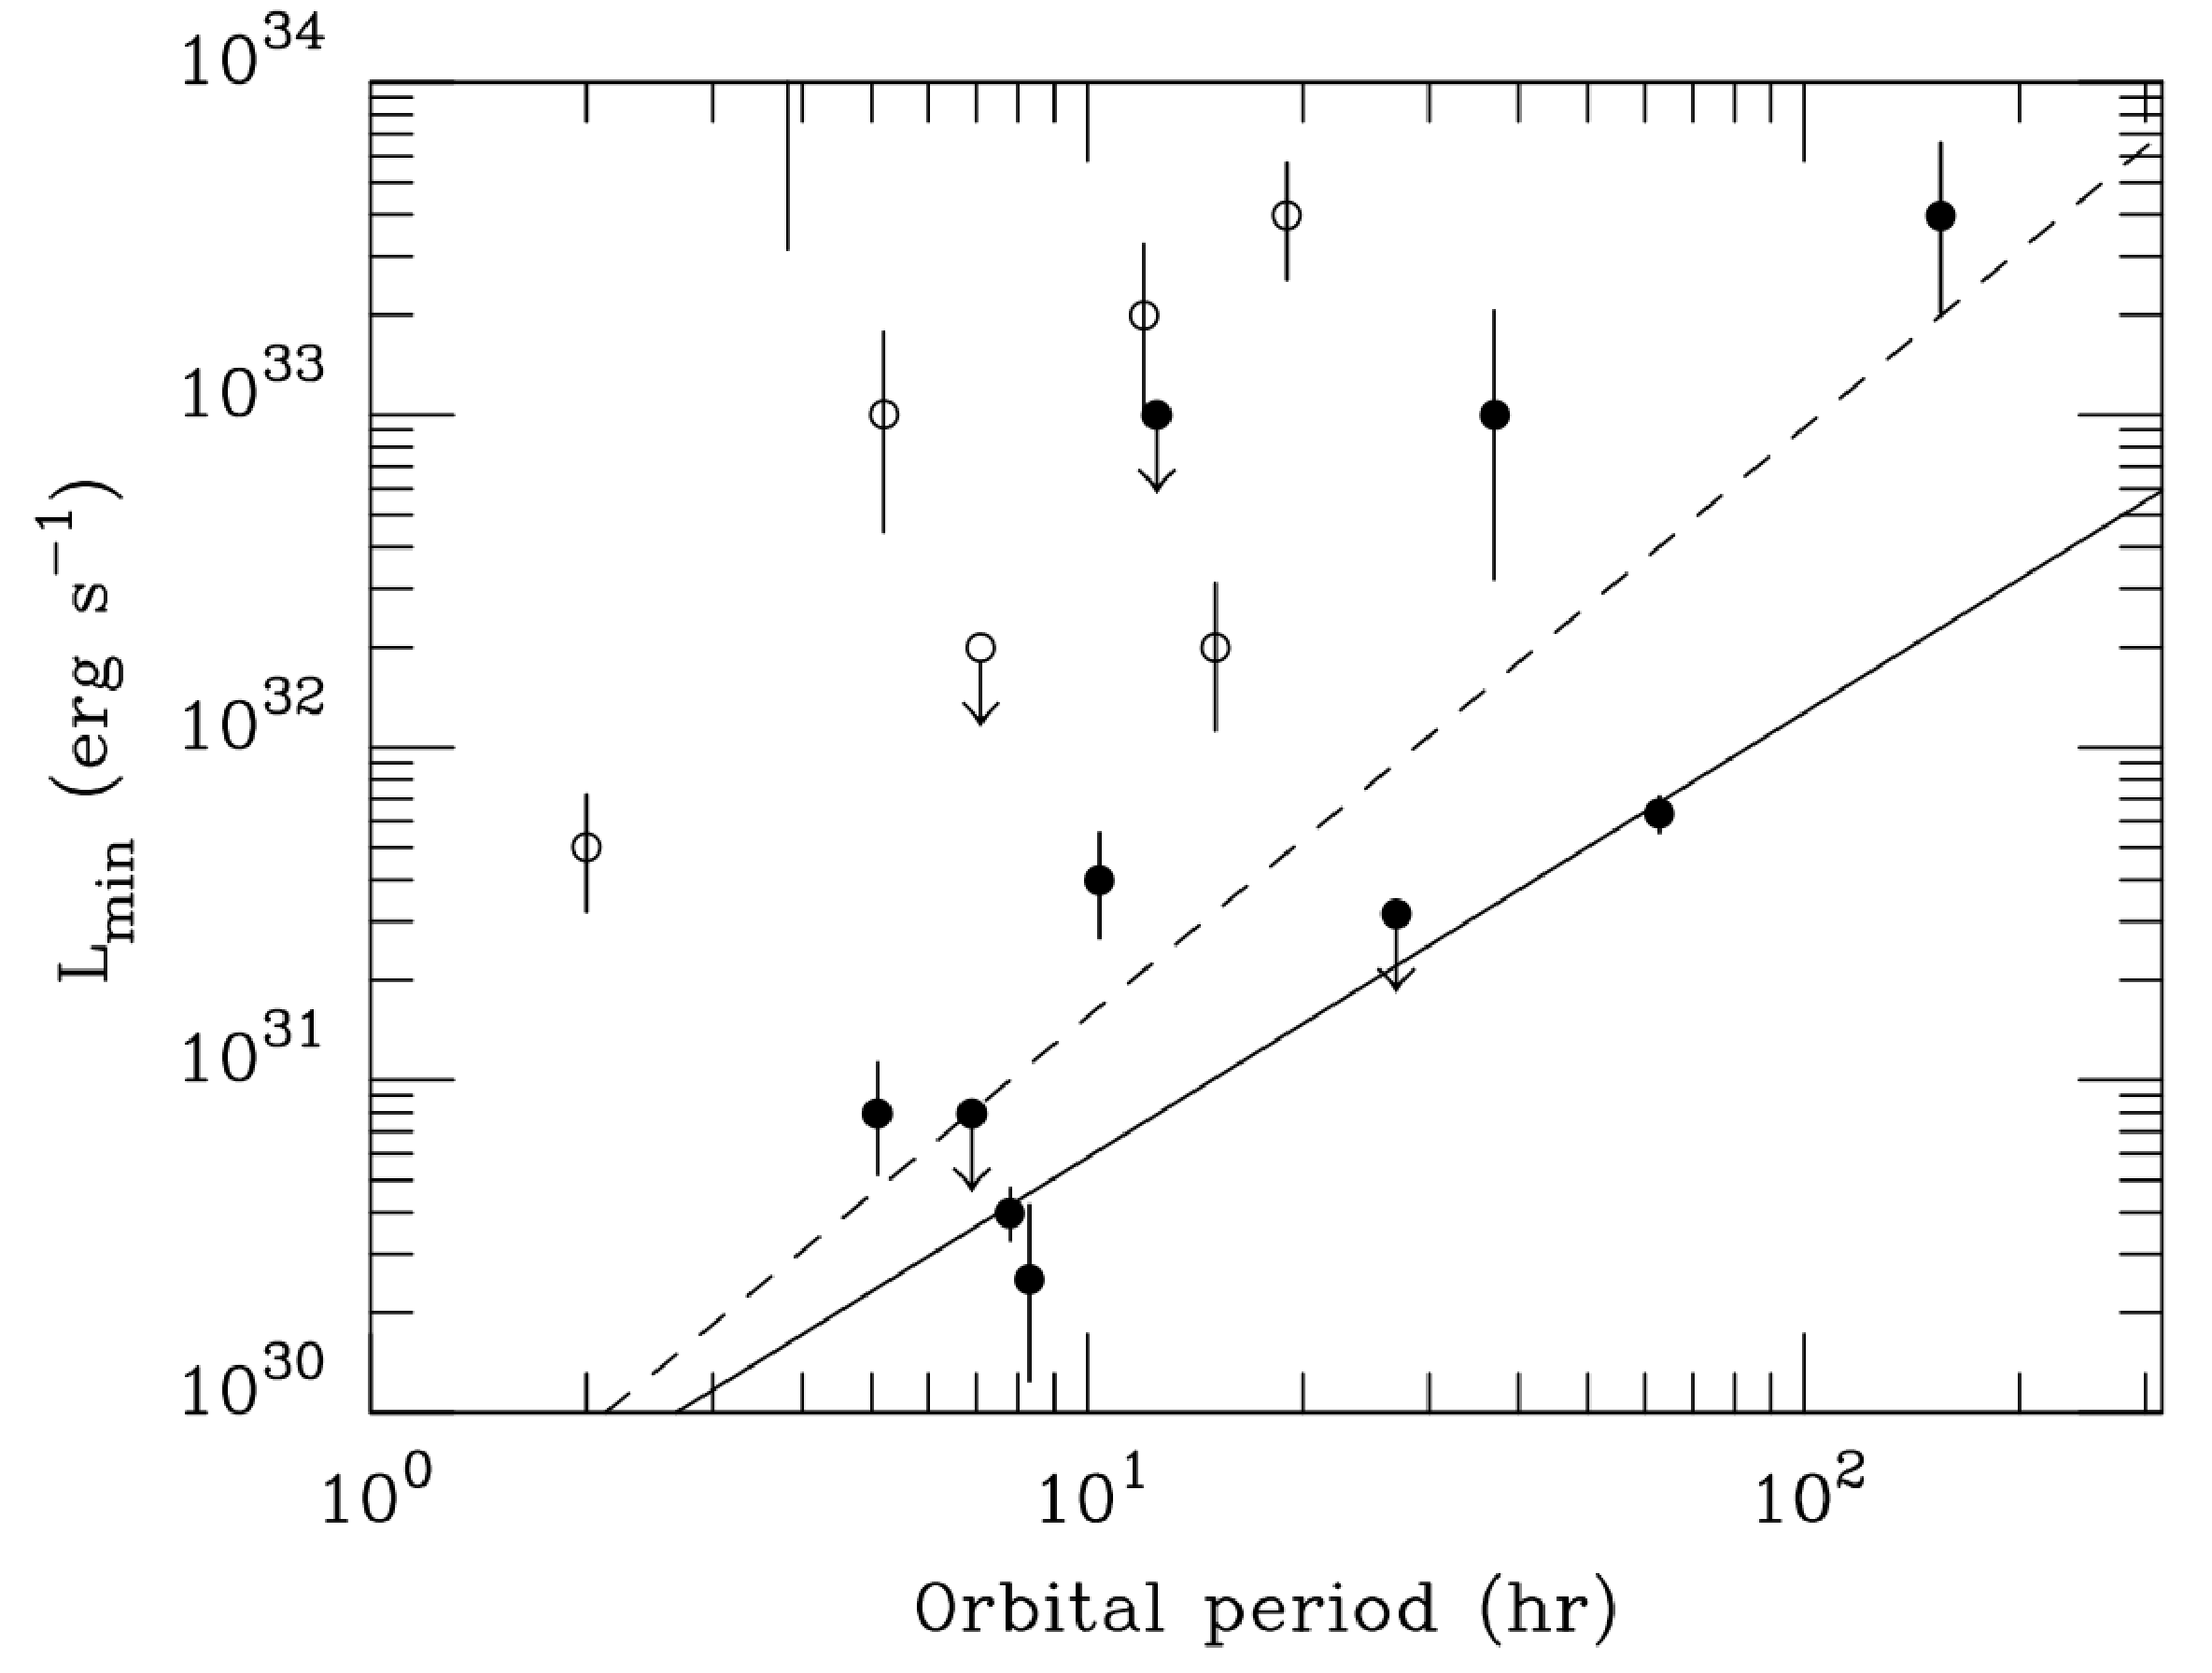
\includegraphics[width=0.7\textwidth]{HighEnergy/Hameury_03}
   \caption{XRBs in quiescence (Hameury et al. 2003). Open circles represent neutron stars and filled circles represent black holes. }
\label{fig:NsBh}
\end{figure}

   \item Typical time scales

\begin{enumerate}[1)]
   \item Signal propagation:
   
\begin{eqnarray}
   \tau_{visc} &\sim& \frac{M}{\dot{M}} \sim \rho \frac{R^{2}H}{\Sigma \nu} \sim \frac{\Sigma R^{2}}{\Sigma \nu} \nonumnext
               &\sim& \frac{R^{2}}{\nu} \approx 5\times 10^5 ~ R_{10}^{10/8} M^{2/8}\, \dot{M}_{16}^{-3/10} \alpha^{-4/5}
\end{eqnarray}
Recall: $\nu$ has units length$^2$/time.

$\tau_{visc}$ is the time it takes for the disk to be drained completely if the accretion source turns off
(\eg, mass transfer from companion star)

   \item Thermal (Kelvin-Helmholtz) time:

\begin{eqnarray}
   \tau_{th} &\sim& \frac{E_{th}}{\dot{E}} \sim \frac{\rho c_{s}^{2} R^{2} H}{GM\dot{M}/R} \sim \frac{\Sigma c_{s}^{2}R^{3}}{CM\Sigma \nu} \nonumnext
             &\sim& \frac{\Sigma c_{s}^{2}}{\Sigma \nu \Omega^{2}} \sim \frac{c_{s}^{2}R^{2}}{\nu R^{2}\Omega^{2}} \sim \frac{c_{s}^{2} R^{2}}{\nu v_{\phi}^2}
\end{eqnarray}
\begin{equation}
   \therefore \tau_{th} \sim \tau_{visc} \left( \frac{c_{s}^{2}}{v_{\phi}^{2}} \right) \ll \tau_{visc}
\end{equation}

$\Rightarrow$ Thermal evolution much more rapid than viscous for thin disks.
\end{enumerate}

   \item Non-local dissipation - corona

\begin{figure}[!htbp]
   \centering
   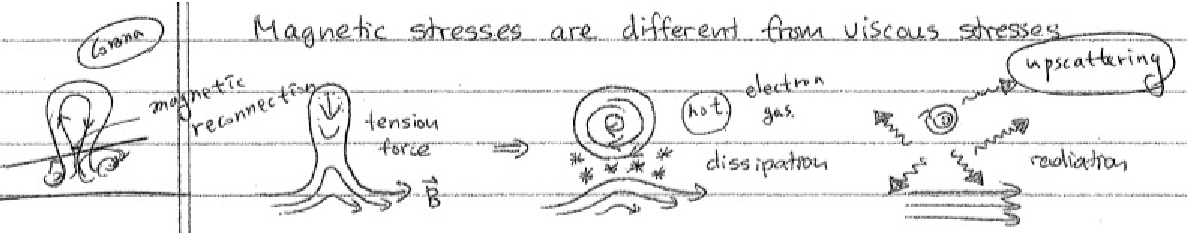
\includegraphics[width=\textwidth]{HighEnergy/note01}
   \caption{Magnetic stresses are different from viscous stresses}
\end{figure}

If viscosity is magnetic, dissipation will be dominated by reconnection.

$\Rightarrow$ Dissipation independent of $\rho$, field lines can rise out of disk and dissipate.

$\Rightarrow$ A layer of hot, low density gas will form above the disk - a ``coronae'' (See the Sun)

Emission: Soft photons from disk are Compton-upscattered (See fig.(\ref{fig:coronae}))
\begin{figure}[!htbp]
   \centering
   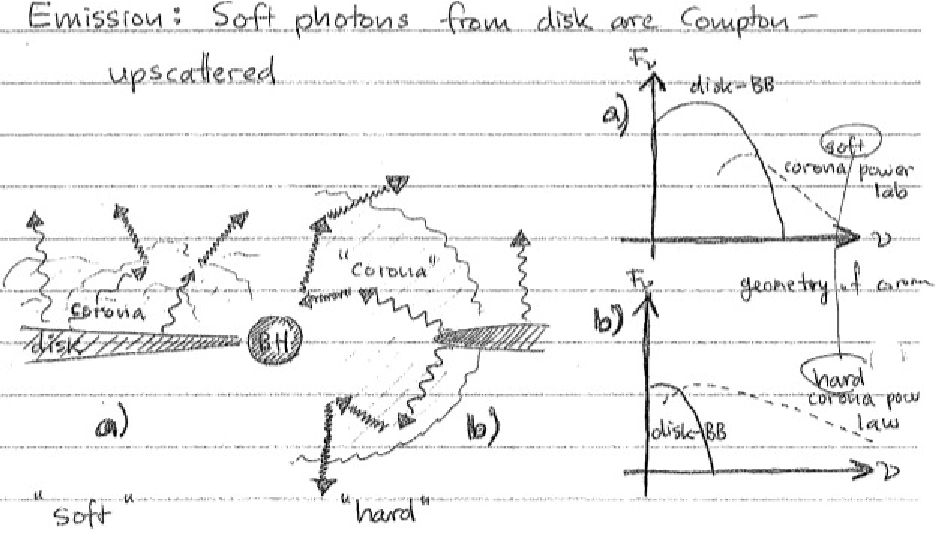
\includegraphics[width=\textwidth]{HighEnergy/note02}
   \caption{Emission: Soft photons from disk are Compton-upscattered}
   \label{fig:coronae}
\end{figure}

\end{enumerate}

\subsubsection{Viscosity Shear Stress: Spherical Coordinate}

The tensors are working on both the momentum equation for angular momentum transport and 
the energy equation for viscous heating \cite{Stone:99}:

\begin{equation}\label{eq:mom}
    \rho \frac{d \vec{v}}{d t} = - \nabla P - \rho \nabla \Phi + \nabla \cdot \boldsymbol{T}
\end{equation}
\begin{equation}
    \rho \frac{d(e/\rho)}{dt} = -P \nabla \cdot \vec{v} + \boldsymbol{T}^{2}/\mu
\end{equation}
where $\boldsymbol{T}$ is an anomalous stress tensor, and $\mu = \rho \nu$ is the coefficient of shear viscosity,
and $\nu$ is the kinematic viscosity coefficient:
\begin{equation}
    \nu = \frac{\alpha \, c_{s}^{2}}{\Omega_{\rm k}}
\end{equation}
where $c_{s}$ is the sound speed of the medium, $\alpha$ is a conventional parameter for thin
disk model by \cite{Shakura:73}.  and $\Omega_{\rm k}$ is the keplerian angular velocity,
\begin{equation}
    \Omega_{\rm k} = \left( \frac{1}{r} \frac{\partial \Phi}{\partial r} \right)^{1/2},
\end{equation}

In spherical coordinates, the shear stress elements can be expressed as:
\begin{equation}
    \boldsymbol{T}_{r\theta}=\boldsymbol{T}_{\theta r} = 
         \mu \left\{ r \frac{\partial}{\partial r} \left( \frac{v_{\theta}}{r} \right) + \frac{1}{r} \frac{\partial v_{r}}{\partial \theta}  \right\}
\end{equation}
\begin{equation}
    \boldsymbol{T}_{r\phi}=\boldsymbol{T}_{\phi r} = 
         \mu \left\{ r \frac{\partial}{\partial r} \left( \frac{v_{\phi}}{r} \right) + \frac{1}{r \sin{\theta}} \frac{\partial v_{r}}{\partial \phi}  \right\}
\end{equation}
\begin{equation}
    \boldsymbol{T}_{\theta\phi}=\boldsymbol{T}_{\phi\theta} = 
         \mu \left\{ \frac{\sin{\theta}}{r} \frac{\partial}{\partial \theta} \left( \frac{v_{\phi}}{\sin{\theta}} \right) + \frac{1}{r \sin{\theta}} \frac{\partial v_{\theta}}{\partial \phi}  \right\}
\end{equation}
These derived tensors were confirmed by \cite{Okuda:97} (note that there are some typos in the equations of the paper). 
Since we are considering 2-D simulation ($r,\theta$), $\partial/\partial{\phi}$ term in the equations above can be neglected.

The divergence of a tensor is 
\begin{equation}
    \nabla \cdot \boldsymbol{T} = \frac{\partial T_{ij}}{\partial x_{j}} \, \boldsymbol{e}_{i}.
\end{equation}
Using this tensor calculus, the tensor term in eq.~(\ref{eq:mom}) can be expressed as
\begin{align}\label{eq:fullT}
    \nabla \cdot \boldsymbol{T} =& 
    \left\{ \frac{\partial T_{rr}}{\partial r} + \frac{1}{r}\frac{\partial T_{r\theta}}{\partial \theta} 
    + \frac{1}{r\sin{\theta}}\frac{\partial T_{r\phi}}{\partial \phi} 
    + \frac{2\,T_{rr}+\cot{\theta}\,T_{r\theta}-T_{\theta\theta}-T_{\phi\phi}}{r}  \right\}\,\hat{r} \\ 
   &+ \left\{ \frac{\partial T_{\theta r}}{\partial r} + \frac{1}{r}\frac{\partial T_{\theta\theta}}{\partial \theta} 
    + \frac{1}{r\sin{\theta}}\frac{\partial T_{\theta\phi}}{\partial \phi} 
    + \frac{T_{r\theta}+2T_{\theta r}+\cot{\theta}(T_{\theta\theta}-T_{\phi\phi})}{r}  \right\}\,\hat{\theta}  \nonumnext
   &+ \left\{ \frac{\partial T_{\phi r}}{\partial r} + \frac{1}{r}\frac{\partial T_{\phi\theta}}{\partial \theta} 
    + \frac{1}{r\sin{\theta}}\frac{\partial T_{\phi\phi}}{\partial \phi} 
    + \frac{T_{r\phi}+2T_{\phi r}+\cot{\theta}(T_{\theta\phi}+T_{\phi\theta})}{r}  \right\}\,\hat{\phi}.  \nonumber 
\end{align}
Applying $T_{r\theta}=T_{\theta r}$, $T_{r\phi}=T_{\phi r}$, $T_{\theta\phi}=T_{\phi\theta}$ and
ignoring normal stress terms and $\partial/\partial \phi$ terms, the eq.~(\ref{eq:fullT}) can be rewritten as

\begin{align}\label{eq:partT}
    \nabla \cdot \boldsymbol{T} =& 
    \left\{ \frac{1}{r}\frac{\partial T_{r\theta}}{\partial \theta} 
    + \frac{\cot{\theta}\,T_{r\theta}}{r}  \right\}\,\hat{r} \\ 
   &+ \left\{ \frac{\partial T_{r \theta}}{\partial r} 
    + \frac{3\,T_{r\theta})}{r}  \right\}\,\hat{\theta}  \nonumnext
   &+ \left\{ \frac{\partial T_{r \phi}}{\partial r} + \frac{1}{r}\frac{\partial T_{\theta\phi}}{\partial \theta} 
    + \frac{3\,T_{r\phi}+2\,\cot{\theta}\,T_{\theta\phi}}{r}  \right\}\,\hat{\phi}.  \nonumber 
\end{align}

The angular momentum transport ($\hat{\phi}$) by the stress tensor can be explained by several mechanisms:
magneto-rotational instability, gravitational instability, and asymmetric gravitational torque.
However, the way of momentum loss in other components is not clear. 

\bigskip
\subsection{Jets}

In accretion physics, the motivation was predominantly theoretical in nature. (\ie, we knew
material must fall into the potential wall of the compact object, conserving angular momentum
$\Rightarrow$ accretion), supported by a body of circumstantial evidence (spectra, luminosity,
variability). We know why accretion happens.

In jet physics, the situation is reversed. We know that jets exist primarily from an observational 
point of view (unlike accretion flows, they are resolved), but we don't know why.
\begin{empheq}[innerbox=\fbox,
left=\Rightarrow]{align}
~~\textrm{Phenomenological approach to understanding jets} \nonumber
\end{empheq}

\subsubsection{Phenomenology}

   \begin{enumerate}[a)]
      \item jets in astrophysical systems 
      \begin{itemize}
          \item classic radio loud AGN ($\ge$ 10\%)
          \item X-ray binaries
             \subitem - black holes ~~(essentially all)
             \subitem - neutron stars (Z-sources)
             \subitem - white dwarfs ~(some CVs)
          \item Gamma ray bursts (100\%)
          \item Proto-stars
          \item Pulsars ?
      \end{itemize}
   The ultimate test for the presence of a jet is still the resolved image of an elongated (\ie, collimated)
   structure pointing away from a point source.

\begin{figure}[!htbp]
   \centering
   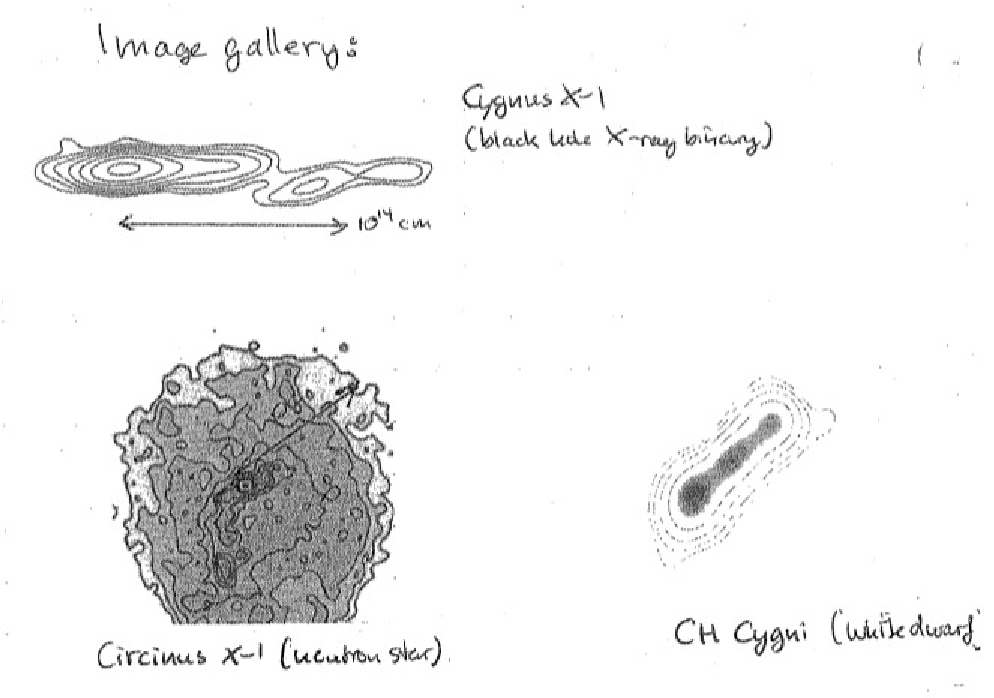
\includegraphics[width=0.7\textwidth]{HighEnergy/note03}
   \caption{Top:Cygnus X-1, bottom-left: Circinus X-1 (neutron star), bottom-right: CH Cygni (White dwarf)}
\end{figure}

\textbf{Morphology (See table (\ref{tab:agn}))}

   \begin{table}[ht]
   \caption{Fanaroff-Riley classification of radio galaxies (See fig.(\ref{fig:FR}))}
   \centering
   \begin{tabular}{cc}
   \hline \hline
   Type I & Type II \\ [0.5ex]
   \hline
   Brighter on smaller scales & Brighter on larger scales \\
   Jet brighter than lobe     & Jet dimmer than lobe      \\ 
   Often two-sided jets       & Most often one-sided jets \\
   Often bent jets            & Straight jets             \\ [1ex]
   \hline
   \end{tabular}
   \label{tab:agn}
   \end{table}

\begin{figure}[!htbp]
   \centering
   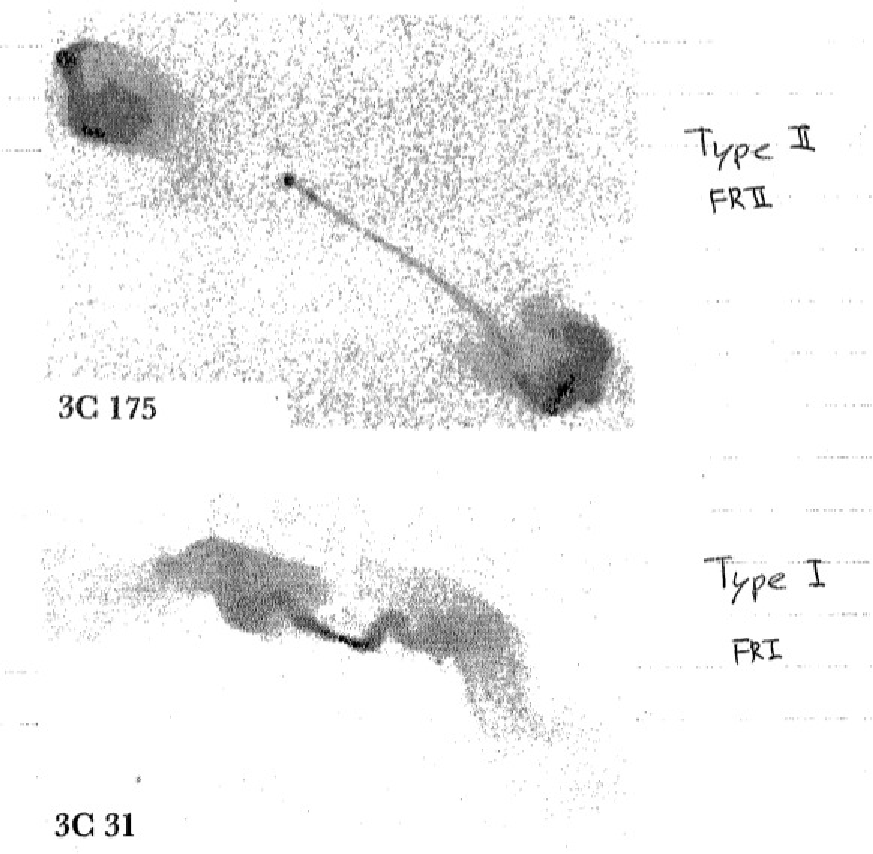
\includegraphics[width=0.7\textwidth]{HighEnergy/note04}
   \caption{Top: FRII galaxy, bottom: FRI galaxy}
\label{fig:FR}
\end{figure}

\begin{figure}[!htbp]
   \centering
   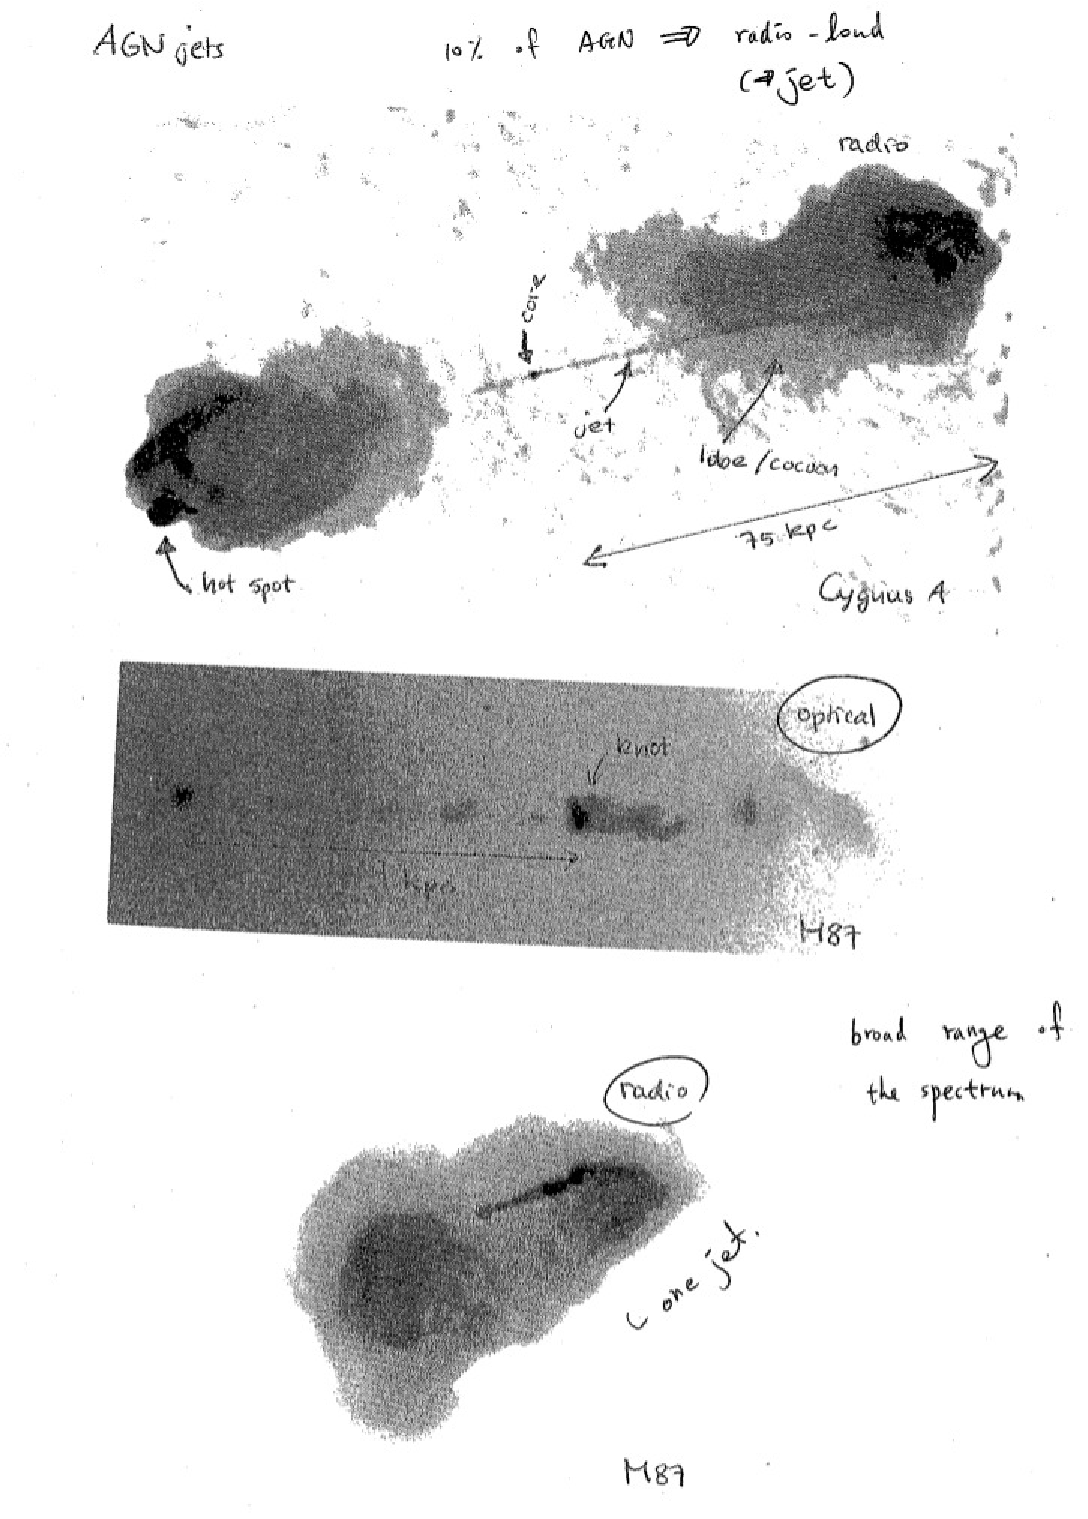
\includegraphics[width=\textwidth]{HighEnergy/note05}
   \caption{AGN jets}
\label{fig:angjets}
\end{figure}

\begin{figure}[!htbp]
   \centering
   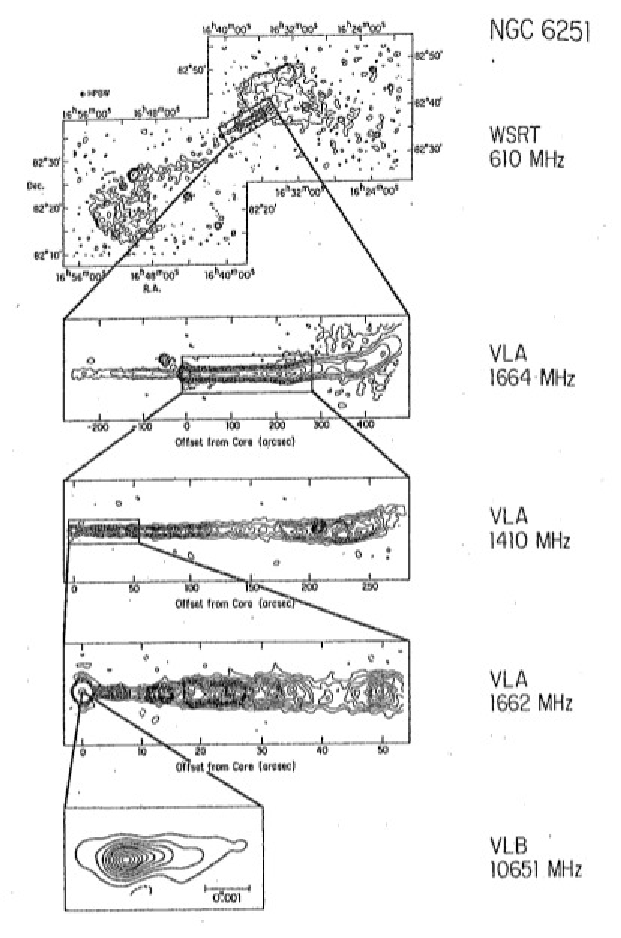
\includegraphics[width=0.9\textwidth]{HighEnergy/note06}
   \caption{The FRI radio galaxy NGC 6251 at a succession of resolution and frequencies (courtesy A. Bridle).
           Although small displacements occur from scale to scale, overall the jet retains a remarkably constant
           alignment over a dynamic range in length scale of $10^{6}$!}
\label{fig:ngc6251}
\end{figure}

   \item Quantification:
   
   Since AGN jets are the best studied species of relativistic jet, we will concentrate on them for a moment.

   \textbf{Spectra:}

\begin{figure}[!htbp]
   \centering
   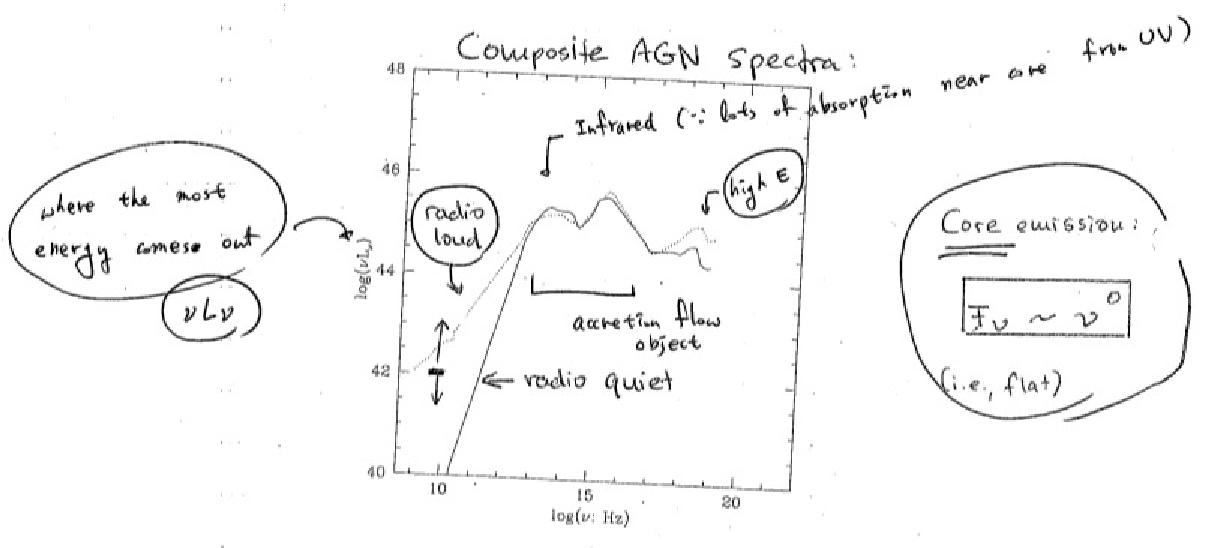
\includegraphics[width=\textwidth]{HighEnergy/note07}
   \caption{Composite AGN Spectra. Dotted line represents radio-loud AGN and solid line represents radio-quiet AGN.}
\label{fig:AGNspectra}
\end{figure}

   $\nu L_{\nu}$ spectrum indicates where the most energy comes out (See fig.(\ref{fig:AGNspectra})).

   ``Radio loud'' AGN: Flat radio spectra from the nuclear region. $F_{\nu} \sim \nu^{0}$

   Radio loudness, 

\begin{equation}
   R = \frac{L_{radio}}{L_{bol}} \simeq \frac{L_{5Ghz}}{L_{B}}
\end{equation}
where $L_{B}$ is luminosity in B-band. We classify AGN as Radio loud, when $R > 2\times 10^{-4}$.

$L_{radio} \sim {\rm few} \times 10^{30}$ to ${\rm few} \times 10^{42}\,\unitpower$

\textbf{BL-Lac objects and ``blazars''}

Some sources are completely dominated by jet emission, \ie, the broad emission lines are hardly seen.

BL-Lacertae-objects and ``blazars''

\begin{figure}[!htbp]
   \centering
   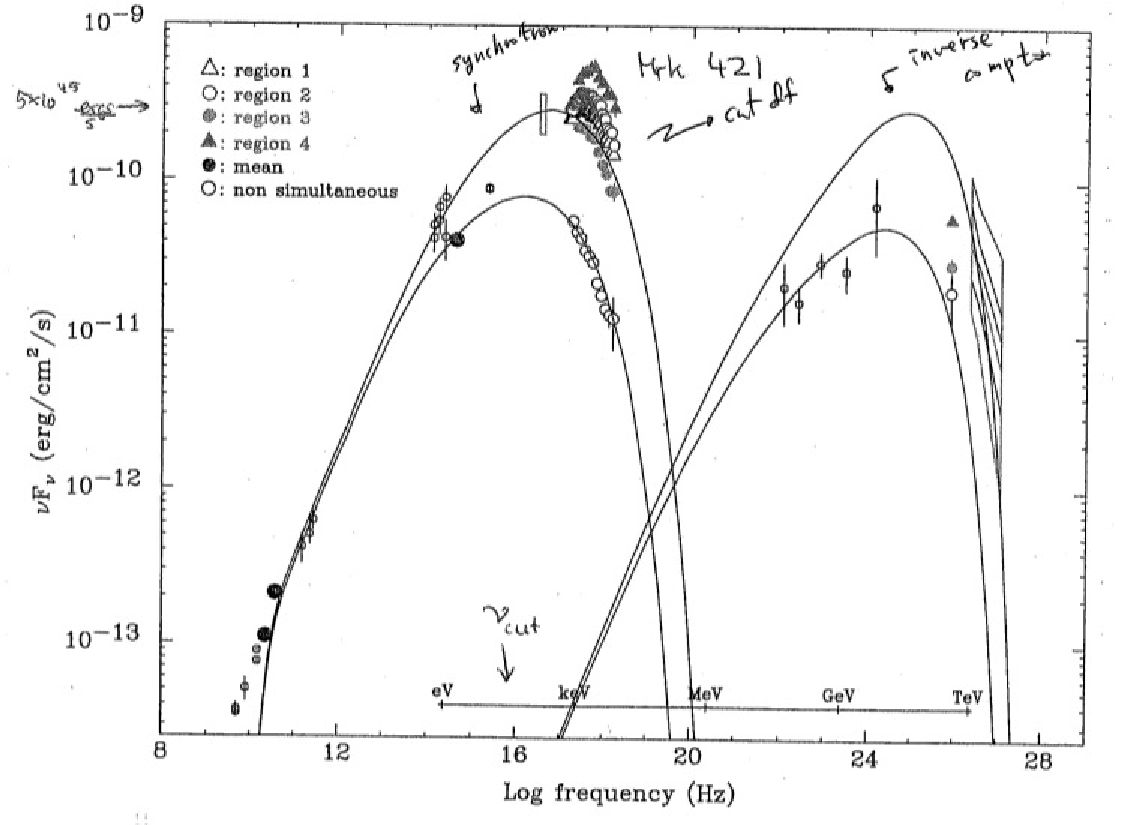
\includegraphics[width=0.7\textwidth]{HighEnergy/note08}
   \caption{Spectrum of BL-Lac object}
\label{fig:BLspectrum}
\end{figure}

These objects, fig.(\ref{fig:BLspectrum}), have pure power-law spectrum up to some cut-off frequency $\nu_{cut}$.
Furthermore, they have X-ray \& $\gamma$-ray spectra of the same shape.

\textbf{Extended emission:}
   \begin{itemize}
      \item Jets show radio spectra with index $\alpha \approx 0.6$, where

\begin{equation}
   F_{\nu} \propto \nu^{-\alpha}
\end{equation}
   cf) core emission: $F_{\nu} \propto \nu^{0}$, \ie flat spectrum

      \item Radio lobes show steeper spectra with $\alpha \approx 1-2$, since optically thin relatively to central region.
   \end{itemize}

\textbf{Polarization:}

Jet emission is almost always polarized. The degree of polarization ranges from a few tenths of a percent to almost 70\%.

We observe strongly polarized power-law (non-thermal) emission across the entire electromagnetic spectrum.

Possible processes:

   \begin{enumerate}[1)]
      \item Synchrotron radiation
      \item Inverse Compton emission
   \end{enumerate}

Answer: Both (Synchrotron at low and inverse compton at high frequencies)

This morphological dichotomy is a fundamental property of radio galaxies.

\end{enumerate}

\subsubsection{Evidence for relativistic motion}

\begin{enumerate}[a)]
   \item Proper motion  (super-luminal motion)
\begin{figure}[!htbp]
   \centering
   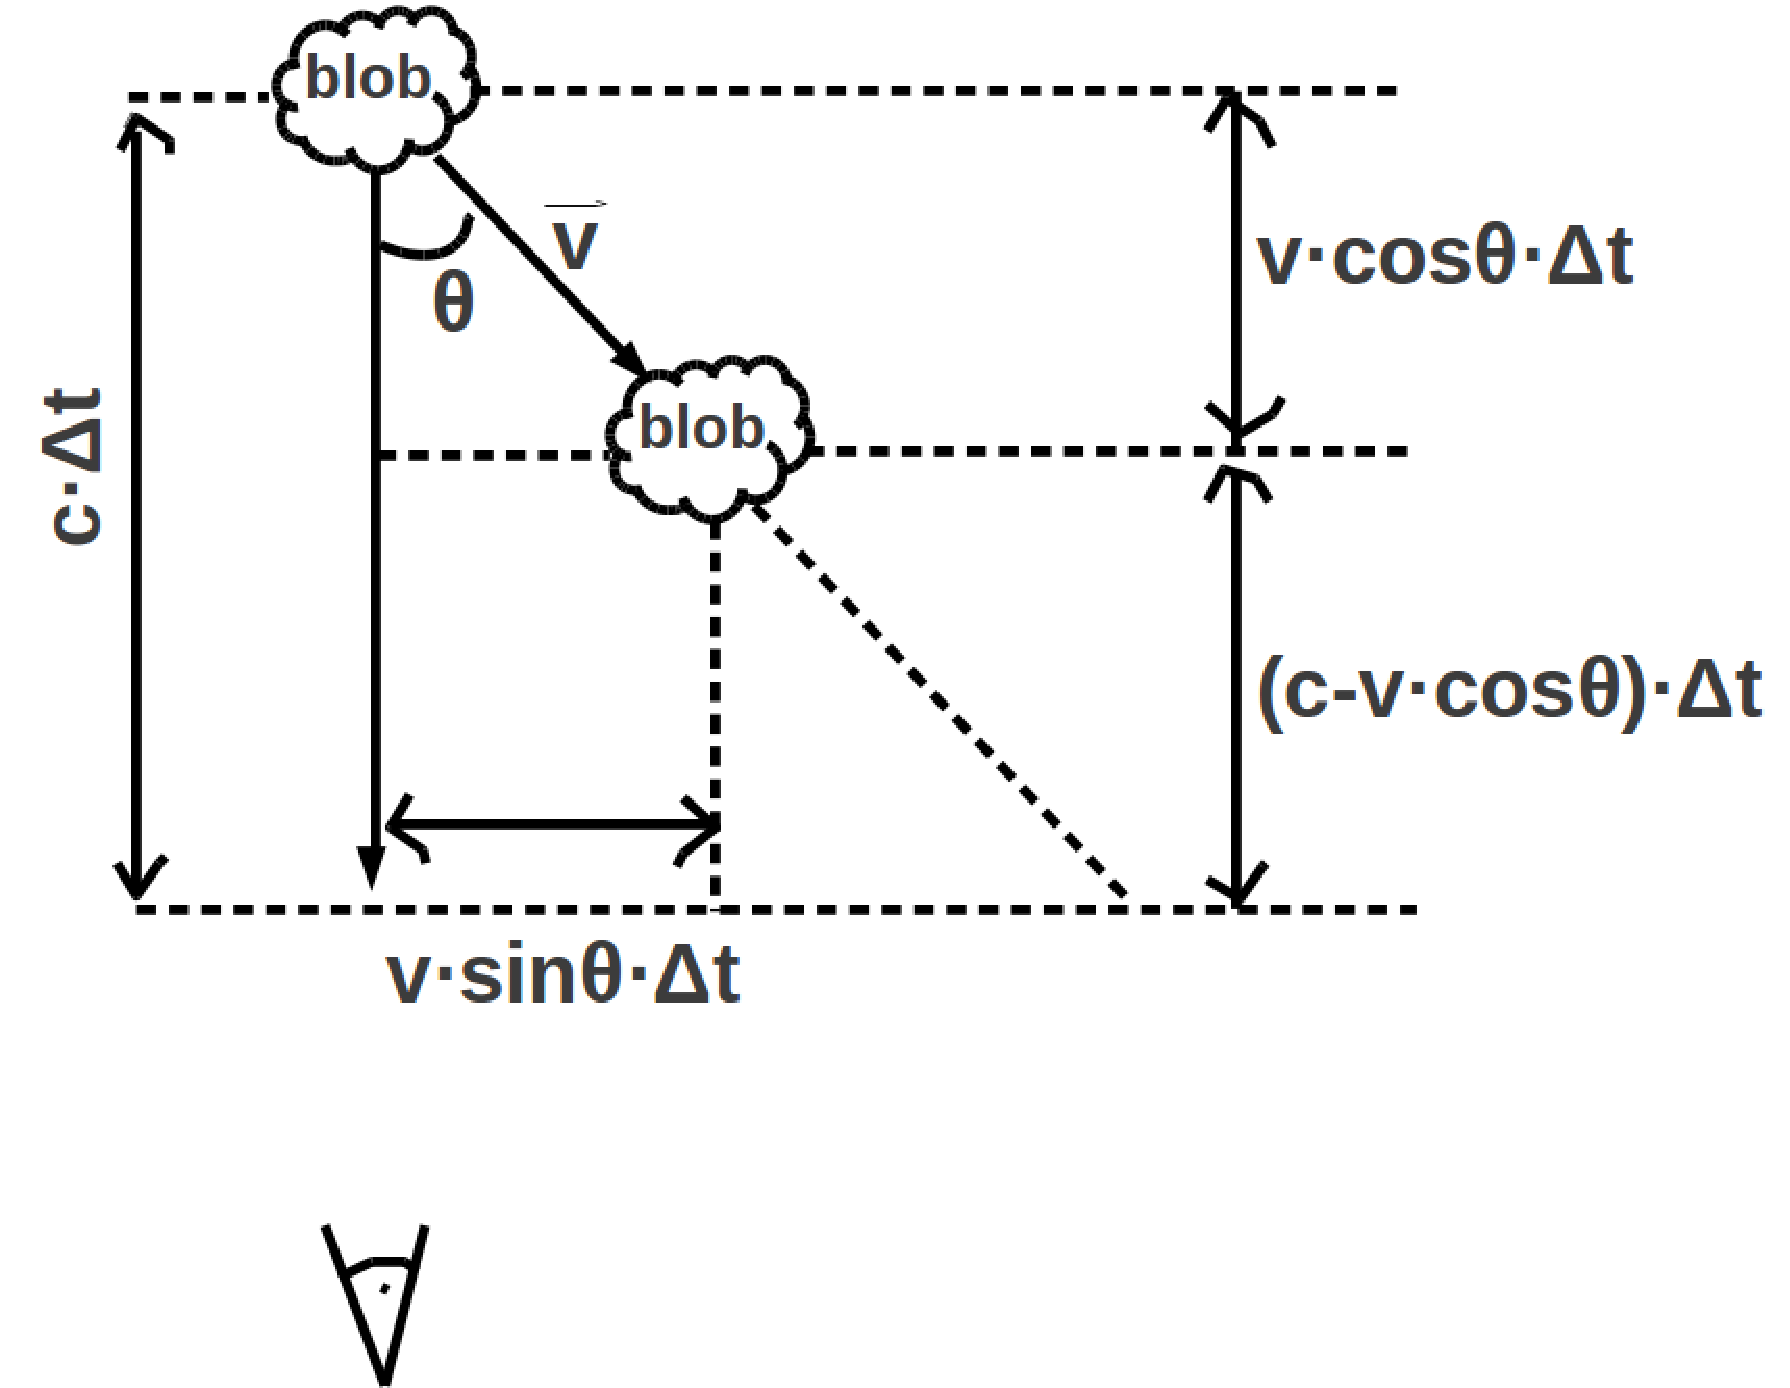
\includegraphics[width=0.7\textwidth]{HighEnergy/superluminal}
   \caption{Super-luminal motion}
\label{fig:superluminal}
\end{figure}

   \begin{enumerate}
      \item perceived distance traveled

\begin{equation}
   \Delta x = v\cdot \sin \theta \cdot \Delta t
\end{equation}
     
      \item perceived time elapsed

\begin{equation}
   \Delta \tau = \frac{\Delta y}{c}  = \frac{(c-v\cdot \cos \theta)\Delta t}{c} = \left( 1-\beta \cos \theta \right)\Delta t 
\end{equation}
   \end{enumerate}

$\Rightarrow$ perceived proper motion:

\begin{empheq}[innerbox=\fbox,
left=\therefore~~]{align}
v_{obs} = \frac{\Delta x}{\Delta \tau} = \frac{v\cdot \sin \theta}{1-\beta \cos \theta}
\end{empheq}
or,
\begin{empheq}[innerbox=\fbox]{align}
\beta_{obs} = \frac{\beta \sin \theta}{1-\beta \cos \theta}
\end{empheq}
Recall $\beta < 1$,
\begin{eqnarray}
   \beta_{obs} = \frac{\beta \sin \theta}{1-\beta(1-\sin^{2} \theta)^{1/2}} \nonumnext
   \Rightarrow ~~ \frac{1}{\beta} = (1-\sin^{2})^{1/2} + \frac{\sin \theta}{\beta_{obs}} > 1 
\end{eqnarray}
\begin{empheq}[innerbox=\fbox,
left=\Rightarrow~~]{align}
\sin \theta < \frac{2 \beta_{obs}}{1+\beta_{obs}} ~~ \textrm{or} ~~ \theta < \frac{2}{\beta_{obs}}~~\textrm{for}~~\beta_{obs} \gg 1
\end{empheq}
Recall
\begin{empheq}[innerbox=\fbox]{align}
\beta \Gamma \ge \beta_{obs}
\end{empheq}
where $\Gamma = \sqrt{1/(1-\beta^{2})}$. Note that $\beta_{obs}$ might not be a physical speed,
\ie, a pattern speed from a moving shock.
Note that Superluminal motion is not a relativistic effect, it is purely a light-travel time effect.
\begin{figure}[!htbp]
   \centering
   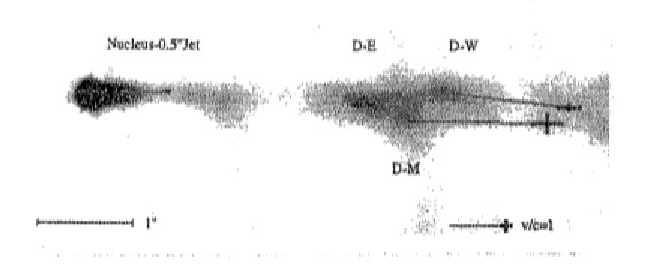
\includegraphics[width=\textwidth]{HighEnergy/note10}
   \caption{M87. $\beta_{obs} \sim 3-5$}
\label{fig:M87}
\end{figure}
Most extreme blazars: $\beta_{obs} \sim 30-50 !$

   \item \textbf{Relativistic Doppler boosting}: relativistic beaming + blue shift

   FRII sources are almost always one-sided. This is easily understood as a consequence of Doppler boosting.

   Assume each source has two equal jets traveling in opposite directions (jet and counter-jet). Each
   emits radiation at a rate $L_{\nu}$ in its own, co-moving frame. Doppler boosting implies that
   the detected luminosity is 

\begin{equation}
   L_{obs} = \delta^{k+\alpha} L_{\nu}
\end{equation}
where $k$ is what kind of object you're looking at, and $\delta$ is the Doppler factor,
\begin{equation}
   \delta = \frac{1}{\Gamma (1-\beta \cos \theta)}
\end{equation}
In case of moving away, $\delta = \frac{1}{\Gamma (1+\beta \cos \theta)}$.
Note that
\begin{empheq}[left=\Rightarrow\empheqlbrace]{align}
   \theta \ll 1~~ &\rightarrow~~ \delta \gg 1 ~~\textrm{for}~ \theta < 1/\Gamma \nonumnext
   \theta \gg 1~~ &\rightarrow~~ \delta \sim 1/\Gamma \ll 1
\end{empheq}
$\alpha$ is the spectral index ($F_{\nu} \propto \nu^{-\alpha}$), and 
\[ \left. \begin{array}{ll}
k=2 & \textrm{(continuous emission)} \\
k=3 & \textrm{(blob-emission)}
\end{array} \right. \]
and $\beta=v/c,~ \Gamma=1/\sqrt{1-\beta^{2}},~\theta$=angle to line-of-sight.
The jet-to-counter-jet brightness ratio is then,
\begin{equation}
   \frac{L_{obs,jet}}{L_{obs,counter-jet}} = \left( \frac{1+\beta \cos \theta}{1-\beta \cos \theta} \right)^{k+\alpha} \equiv l^{k+\alpha}
\end{equation}

Note:
      \subitem 1) $\Gamma$ cancels out ~~~ (convenient)
      \subitem 2) $L$ cancels out ~~~ (distance independence !)
      \subitem 3) $\beta$ and $\theta$ only enter as product $\Rightarrow$ can only measure $\beta \cdot \cos \theta$

\begin{empheq}[innerbox=\fbox]{align}
   \beta\cdot\cos\theta = \frac{l-1}{l+1}
\end{empheq}
Since we know $\beta<1$ and $\cos \theta \le 1$:
\begin{equation}
   \beta \ge \frac{l-1}{l+1} ~~~\textrm{and}~~~ \cos\theta > \frac{l-1}{l+1}
\end{equation}

Example: M87

$~~~~~ L_{obs,jet} \ge 380 \cdot L_{obs,counter-jet}$ \\
$~~~~~ \Rightarrow ~~ l_{obs} \ge 11$ \\
$~~~~~ \Rightarrow ~~ \beta \ge 0.83 ~~~\textrm{and}~~~ \theta < 34^{\circ}$ \\
$~~~~~~ \textrm{where}~ \Gamma \ge 2$ 

   \item Variability
   
   Some radio loud AGN (\eg, blazars) vary on time scales of days and shorter across the entire spectrum. 

   Causality implies a source size limit of 
\begin{equation}
   \Delta r \le c\cdot \Delta t \sim 10^{16} \rm\,cm
\end{equation}
Note: the observed time $\Delta t_{obs}$ is shorter by a factor $\delta^{-1}$ than the co-moving time,
\begin{equation}
   \Delta t_{obs} = \Delta t_{co} / \delta
\end{equation}
The emission is polarized and follows a roughly flat power-law $\Rightarrow$ optically thick synchrotron emission.
For a typical luminosity of $10^{42} \,\unitpower$ at 5 Ghz, the surface brightness of the emission (observed) is
\begin{equation}
   S_{\nu,obs} = \frac{L_{\nu,obs}}{(4\pi)(\pi \Delta r^{2})} = 0.05 \,\rm erg\,cm^{-2}\,s^{-1}Hz^{-1}Sr^{-1}
\end{equation}
which corresponds to a brightness temperature of 
\begin{equation}
   T_{b,obs} = \frac{c^{2}}{2\nu^{2}k} \cdot S_{\nu} \approx 10^{16} K ~~~(\textrm{not reasonable})
\end{equation} 
Recall from synchrotron theory of self-absorbed sources:
\begin{equation}
   S_{\nu} = \frac{j_{\nu}}{\alpha_{\nu}} \propto B^{-1/2} \nu^{5/2}
\end{equation}
where $j_{\nu}$ is emissivity and $\alpha_{\nu}$ is absorption coefficient. Up to some maximum frequency
$\nu_{peak}$, so the bolometric radiation energy density is
\begin{equation}
   u_{rad} \sim \frac{S_{peak}}{c} \propto B^{-1/2} \nu_{peak}^{5/2}
\end{equation}
while the magnetic energy density follows 
\begin{equation}
   u_{B} = \frac{B^2}{8\pi} \propto B^{2}
\end{equation}
Now, recall from synchrotron and inverse Compton theory that losses are proportional to $u_{B}$ and $u_{rad}$,
respectively. If $u_{rad}$ is ever larger than $u_{B}$, Compton losses grow exponentially (instability) and cool
the particle distribution to the point where $u_{rad} \le u_{B}$ again (this is called the ``Compton catastrophe'')

$\Rightarrow$ In synchrotron emitting sources: $u_{B} \ge u_{rad}$

We can re-write this, using $u_{rad} \sim B^{-1/2}\nu_{peak}^{5/2}$:
\begin{eqnarray}
   u_{rad} / u_{B} &<& \rm const \nonumnext
   \Rightarrow B^{-5/2}\, \nu_{peak}^{5/2} &<& \rm const \nonumnext
   B^{-1/2}\, \nu_{peak}^{1/2} &<& \rm const ~~~\equiv~~~ T_{max}
\end{eqnarray}
Plugging the expression for $S_{peak}$ in, this gives
\begin{equation}
   S_{peak} \sim B^{-1/2}\nu_{peak}^{5/2} < T_{max}\nu_{peak}^{2}
\end{equation}
or
\begin{equation}
   {T_{B,peak}} = \frac{S_{peak}c^{2}}{2\,k\,\nu_{peak}^{2}} < T_{max} \approx 10^{12}\,K
\end{equation}
Thus, the brightness temperature of a synchrotron emitting source is limited to 
\begin{equation}
   T_{B} < 10^{12}\, K
\end{equation}

The only way to bring the observed $10^{16} \rm\,K$ in line with this limit is relativistic motion:

   \subitem 1) ~~$\Delta r_{obs} \propto \Delta t_{obs} \propto \Delta t \cdot \frac{1}{\delta} $
   \subitem 2) ~~$\nu_{obs} \propto \nu\cdot \delta$
   \subitem 3) ~~$L_{\nu,obs} \propto L_{\nu}\cdot \delta^{k+\alpha}$

   \subitem $\Rightarrow ~~ T_{obs} \propto \delta^{k+\alpha} \sim \delta^{3}$
   \subitem \textbf{$\Rightarrow ~~\delta \sim 10^{4/3} \sim 20 $}
               
   \item Physical parameters

   Given a physical size and luminosity, we can use synchrotron theory to constrain the physical conditions in the source.

   Recall:

\begin{equation}
   j_{\nu} \approx 10^{-18} \, p\,B^{(p+1)/2}\,\nu_{5GHz}^{-(p-1)/2} \, erg\,cm^{-3}\,s^{-1}Hz^{-1}
\end{equation}
where p is pressure density in relativistic particles ($\united$).

   Example: M87, ``knot A''

   ~~~~ $L_{5Ghz} \approx 5\times10^{29} {\rm\,erg\,s^{-1}Hz^{-1}} \cdot \delta^{-2-\alpha}$

   ~~~~ size: $\Delta r \approx \rm 100 pc$

   ~~~~ $\rightarrow ~~ j_{5Ghz} \approx 4\times10^{-33} \,{\rm erg\,cm^{-3} \,s^{-1} Hz^{-1}} ~~\delta^{-2-\alpha}$ 

   ~~~~ $\rightarrow ~~ p \, B^{1.5} \approx 4\times 10^{-15} \delta^{-2-\alpha}$


   ~~~~ Without a way to measure B directly, we usually proceed to make the (usually poorly justified) assumption of equipartition:

\begin{eqnarray}
   p &\approx& \frac{B^{2}}{8\pi} \\
   \rightarrow p &\approx&  2\times10^{-10} \,erg\,cm^{-3} \delta^{-10/7} \nonumnext
   B &\approx& 100 \, \mu G ~\delta^{-5/7} \nonumber
\end{eqnarray}
We also know that $\Gamma \sim 5$
So roughly,
\begin{empheq}[innerbox=\fbox]{align}
   L_{kin} &\sim \left( 4p+B^{2}/4\pi \right) \pi \Delta r^{2} \Gamma^{2} \beta^{2} c \\ 
           &\sim 3\times 10^{43} \, erg\,s^{-1}
\end{empheq}
(Note: this is just an illustrative example, the numbers are order-of-magnitude accurate only.)

M87 is an FRI source, which is consistent with this kind of power estimate.

Recall from accretion section: $\dot{M}_{\rm Bondi} \sim 0.03 \,\unitmfluxsol$

\begin{empheq}[innerbox=\fbox]{align}
   L_{\rm Bondi} \sim 2\times 10^{43}\, \unitpower
\end{empheq}

\end{enumerate}

\textcolor{red}{compton scattering 
inverse compton scattering}

\bigskip
\subsection{Binary System}

\subsubsection{Kepler's Law}

\noi 1. The orbit of every planet is an ellipse with the sun at one of two foci.
\begin{equation}
   r = \frac{p}{1+\epsilon \cos \theta} \nonumber
\end{equation}
\noindent where p=b$^{2}$/2 (semi-latus rectum), $\epsilon = \sqrt{1-(b/a)^{2}}$ (eccentricity).

\noi 2. A line joining a planet and the sun sweeps out equal area during equal intervals of time.
\begin{equation}
   \frac{d}{dt}\left( \frac{1}{2} r^{2}\theta \right) = 0. \nonumber
\end{equation}

\noi 3. The square of the orbital period of a planet is directly proportional to the cube of the 
semi-major axis of its orbit.
\begin{equation}
   T^{2} = \frac{4\pi^{2}a^{3}}{\textrm{GM}}. \nonumber
\end{equation}

\noi 4. Center of Mass
\begin{equation}
    r_{1}M_{1} = r_{2}M_{2}
\end{equation}
Therefore,
\begin{equation}
    r_{1} = \frac{M_{2}}{M_{1}+M_{2}}\,r
\end{equation}
or,
\begin{equation}
    r_{2} = \frac{M_{1}}{M_{1}+M_{2}}\,r
\end{equation}
where $r = r_{1}+r_{2}$. In this context, the Kepler's law can be expressed as,
\begin{equation}
    \omega^{2} = \frac{G\left( M_{1}+M_{2} \right)}{a^{3}},
\end{equation}
where $\omega = 2\,\pi/T$.

\noi 5. Inclination angle: $i$
If the normal vector of the orbital plane is inclined to the line of sight by an angle $i$, the 
Doppler velocity amplitudes we measure will be 
\begin{equation}
    |v_{1obs}| = |v_{1}|\sin{i}, ~~~ |v_{2obs}| = |v_{2}|\sin{i}.
\end{equation}
Then,
\begin{equation}
    \frac{M_{2}^{3}}{(M_{1}+M_{2})^{2}}\sin^{3}{i} = \frac{\tau |v_{1obs}|^{3}}{2\pi\,G},
\end{equation}
where $\tau = 2\pi\,r_{1}/|v_{1}| = 2\pi\,r_{2}/|v_{2}|$. The detailed derivation is in \cite{Maoz}.

\subsubsection{Tidal force}
\begin{equation}
   dF_{\textrm{Tidal}} = \frac{2 G M m dr}{r^{3}} \nonumber
\end{equation}

